%\documentclass[first,firstsupp,handout,compress,notes,navigation]{ETHclass}
%\documentclass[first,firstsupp,handout,lastsupp]{ETHclass}
\documentclass[first,firstsupp,lastsupp,handout,last,hyperref,table]{ETHclass}
%\documentclass[first,firstsupp]{ETHclass}
\usepackage{etex}

\usepackage{adjustbox}
\usepackage{amsmath}
\usepackage{amssymb}
\usepackage{animate}
\usepackage{booktabs}
\usepackage{charter}
\usepackage{enumitem}
\usepackage{etoolbox}
\usepackage{ifthen}
\usepackage{longtable}
\usepackage{mathrsfs}
\usepackage{multicol}
\usepackage{pgf}
\usepackage{pgfplots}
\usepackage{pifont}
\usepackage{ragged2e}
\usepackage{standalone}
\usepackage[caption=false]{subfig}
\usepackage{tabularx}
\usepackage{tikz}
\usepackage{verbatim}
\usepackage{xcolor}
\usepackage{hyperref}

\pgfplotsset{compat=1.7}

\setbeamertemplate{navigation symbols}{}
\usetikzlibrary{arrows,decorations.pathreplacing,positioning,shapes,shadows}

%\usepackage[style=numeric-comp]{biblatex}

%\usepackage{lipsum}

%\usetikzlibrary{fit}
\usetikzlibrary{arrows}
\usetikzlibrary{trees}

% Options for beamer:
%
% 9,10,11,12,13,14,17pt  Fontsizes
%
% compress: navigation bar becomes smaller
% t       : place contents of frames on top (alternative: b,c)
% handout : handoutversion
% notes   : show notes
% notes=onlyslideswithnotes
%
%hyperref={bookmarksopen,bookmarksnumbered} : Needed for menues in
%                                             acrobat. Also need
%                                             pdftex as option or
%                                             compile with
% pdflatex '\PassOptionsToPackage{pdftex,bookmarksopen,bookmarksnumbered}{hyperref} \input{file}'

%\usepackage{beamerseminar}
%\usepackage[accumulated]{beamerseminar}
                                % remove ``accumulated'' option
                                % for original behaviour
%\usepackage{beamerbasenotes}
%\setbeamertemplate{note page}[plain]
%\setbeameroption{notes on second screen}

%\setbeamertemplate{note page}[plain]
\setbeamertemplate{note page}{\ \\[.3cm]
\textbf{\color{blue}Notes:}\\%[0.1cm]
{\footnotesize %\tiny
\insertnote}}
%\setbeameroption{notes on second screen}


%\setbeamertemplate{navigation symbols}{} % suppresses all navigation symbols:
 \setbeamertemplate{navigation symbols}[horizontal] % Organizes the navigation symbols horizontally.
% \setbeamertemplate{navigation symbols}[vertical] % Organizes the navigation symbols vertically.
% \setbeamertemplate{navigation symbols}[only frame symbol] % Shows only the navigational symbol for navigating frames.

\setlayoutscale{0.5}
\setparametertextfont{\scriptsize}
\setlabelfont{\scriptsize}

% \useoutertheme[subsection=false]{miniframes}
% \usepackage{etoolbox}
% \makeatletter
% \patchcmd{\slideentry}{\advance\beamer@xpos by1\relax}{}{}{}
% \def\beamer@subsectionentry#1#2#3#4#5{\advance\beamer@xpos by1\relax}%
% \makeatother

% \makeatletter
%     \newenvironment{withoutheadline}{
%        \setbeamertemplate{headline}{%
% \vspace{15pt}
% }
%     }{}
% \makeatother

\makeatletter
    \newenvironment{withoutheadline}{
         \setbeamertemplate{headline}{%
\vspace{35pt}
}
        %\def\beamer@entrycode{\vspace*{-1.5\headheight}}
    }{}
\makeatother

\newcommand{\Cross}{$\mathbin{\tikz [x=1.4ex,y=1.4ex,line width=.2ex, red] \draw (0,0) -- (1,1) (0,1) -- (1,0);}$}%

\newcommand{\Checkmark}{$\color{green}\checkmark$}

\setbeamerfont{subsection in toc}{size=\tiny}

\makeatletter
\patchcmd{\beamer@sectionintoc}
  {\vfill}
  {\vskip1.5\itemsep}
  {}
  {}
\makeatother

\setbeamertemplate{frametitle continuation}{}

\setbeamertemplate{bibliography entry title}{}
\setbeamertemplate{bibliography entry author}{}
\setbeamertemplate{bibliography entry location}{}
\setbeamertemplate{bibliography entry note}{}

\setbeamercolor*{bibliography entry title}{fg=black}
\setbeamercolor*{bibliography entry author}{fg=black}
\setbeamercolor*{bibliography entry location}{fg=black}
\setbeamercolor*{bibliography entry note}{fg=black}
% and kill the abominable icon
%\setbeamertemplate{bibliography item}{\color{forestgreen}$\blacktriangleright$}
\setbeamertemplate{bibliography item}{\insertbiblabel}
%\setbeamertemplate{bibliography item}{\theenumiv}

\newcommand{\highlightred}[1]{%
  \colorbox{red!50}{$\displaystyle#1$}}

\newcommand{\highlightyellow}[1]{%
  \colorbox{yellow!50}{$\displaystyle#1$}}

\newcommand{\highlightgreen}[1]{%
  \colorbox{green!50}{$\displaystyle#1$}}

\AtBeginSection[]{
  \begin{frame}
  \vfill
  \centering
  \begin{beamercolorbox}[sep=8pt,center,shadow=true,rounded=true]{title}
    \usebeamerfont{frametitle}
\includegraphics[width=2ex]{freccia_trasparente_verde_foresta.png}\hspace{.5ex}~{\LARGE \textsc{\bfseries \insertsectionhead}}\par%
  \end{beamercolorbox}
  \vfill
  \end{frame}
}

\hyphenpenalty=5000
\tolerance=1000

\graphicspath{{figures/}}

\newenvironment{system}{\left\lbrace\begin{array}{@{}l@{}}}{\end{array}\right.}

\newenvironment{subsystem}{\left\lgroup\begin{array}{@{}l@{}}}{\end{array}\right.}

\defbeamertemplate*{title page}{customized}[1][]
{
\usebeamerfont{subtitle}
\usebeamercolor[fg]{subtitle}

\vspace{-1.75cm}

{\flushleft
 \usebeamerfont{title}{\inserttitle}\par
}
\vspace{-.25cm}
{\flushleft
 \usebeamerfont{subtitle}{\small \insertsubtitle} \par
}

%\vspace{-.5cm}

{\flushright
\setbeamercolor{author}{bg=white,fg=Red}
\usebeamerfont{author}{\footnotesize \insertauthor} \par}

\vspace{-.2cm}

{\flushright
\usebeamerfont{institute}{\tiny \insertinstitute}\par }

\vspace{.2cm}

{\centering
\usebeamerfont{date}{\scriptsize \insertdate} \par }

\vspace{0.2in}
}


\begin{document}
\setbeamertemplate{caption}{\raggedright\insertcaption\par}

\title[\textsc{FEM \& the Fiber-Matrix Interface Crack}]{\textsc{Finite Elements Solution of the Fiber-Matrix Interface Crack: Effects of Mesh Refinement and Domain Size}}
\author{ L. Di Stasio$^{1,2}$, Z. Ayadi$^{1}$, J. Varna$^{2}$}
%\institute{ Science et Ing\'enierie des Mat\'eriaux et M\'etallurgie (SI2M), Institut Jean Lamour, Nancy, France\\Department of Engineering Sciences and Mathematics, Division of Materials Science, Lule\aa\ University of Technology, Lule\aa, Sweden}
\institute{$^{1}$EEIGM, Universit\'e de Lorraine, Nancy, France\\$^{2}$Division of Materials Science, Lule\aa\ University of Technology, Lule\aa, Sweden}
\date{DocMASE Summer School, Sarrebr\"ucken (DE) - Nancy (FR), September 11 - 15, 2017}

\begin{frame}[plain]
    \titlepage
\end{frame}

\begin{withoutheadline}
\begin{frame}
\frametitle{Outline}
\justifying
\vspace*{-0.5cm}
% \tableofcontents[hidesubsections]
% \begin{multicols}{2}
% \tableofcontents[hidesubsections]
% \end{multicols}
% \begin{columns}[t]
%         \begin{column}{.5\textwidth}
%             \tableofcontents[sections={1-2}]
%         \end{column}
%         \begin{column}{.5\textwidth}
%             \tableofcontents[sections={3-6}]
%         \end{column}
%     \end{columns}
% \end{frame}
\tableofcontents[hidesubsections]
\end{frame}
\end{withoutheadline}

%\note{}

%\begin{frame}
%\pagediagram
%\end{frame}
%% \note{}

\section[Characterization of Fracture in FRPC]{Characterization of Fracture in FRPC Laminates}

\subsection[Damage in FRPC]{Damage Onset and Propagation in FRPC Laminates}

\begin{frame}
%\vspace*{-1cm}
\frametitle{\small Damage Onset and Propagation in FRPC Laminates}
\vspace{-0.75cm}
\centering
\captionsetup[subfigure]{labelfont=footnotesize}
\begin{figure}[!h]
\centering
\subfloat[\scriptsize By Dr. R. Olsson, Swerea, SE.\label{fig:all-cracks}]{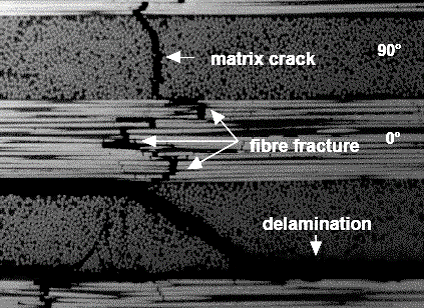
\includegraphics[width=0.46\textwidth]{all-cracks.png}}\quad
\subfloat[\scriptsize By Prof. Dr. E. K. Gamstedt, KTH, SE.\label{fig:transverse-cracks}]{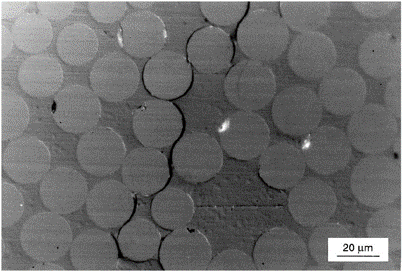
\includegraphics[width=0.5\textwidth]{intralaminar-cracks.png}}
 \caption{A visual definition of intralaminar transverse cracking.}
  \label{fig:intralaminar-cracks}
\end{figure}
\end{frame}

\subsection[Characterization of the Fracture Process]{Characterization of the Fracture Process}

\begin{frame}
%\vspace{-0.5cm}
\frametitle{\small Characterization of the Fracture Process}
\vspace{-0.25cm}
\centering
\scriptsize
\begin{itemize}[label=\ding{212}]
\item Energy Release Rate
\begin{equation*}
G_{m}=G_{m}\left(p_{1},\dots,p_{i},\dots,p_{n}\right)\quad\text{where}\quad G=\frac{\partial W}{\partial A} - \left(\frac{\partial U}{\partial A}+\frac{\partial E_{k}}{\partial A}\right)
\end{equation*}
\item Stress Intensity Factor
\begin{equation*}
K_{m}=K_{m}\left(p_{1},\dots,p_{i},\dots,p_{n}\right)\quad\text{where}\quad \sigma_{m}\sim K_{m}\frac{\alpha}{\left(x-a\right)^{\beta}}\quad\alpha,\beta>0
\end{equation*}
\item J-Integral
\begin{equation*}
J=J\left(p_{1},\dots,p_{i},\dots,p_{n}\right)\quad\text{where}\quad J=\lim_{\varepsilon\to 0}\int_{\Gamma_{\varepsilon}}\left(W\left(\Gamma\right)n_{i}-n_{j}\sigma_{jk}\frac{\partial u_{k}\left(\Gamma,x_{i}\right)}{\partial x_{i}}\right)d\Gamma
\end{equation*}
\item Crack Opening \& Shear Displacement
\begin{equation*}
COD=COD\left(p_{1},\dots,p_{i},\dots,p_{n}\right)\quad\text{and}\quad CSD=CSD\left(p_{1},\dots,p_{i},\dots,p_{n}\right)
\end{equation*}
\end{itemize}
\vspace{5pt}
\begin{equation*}
p_{i}\in\left\{\text{geometry},\text{materials},\text{boundary conditions},\text{loading mode},\text{scale}\right\}
\end{equation*}
\begin{equation*}
m\in\left\{I,II,III,I/II,I/III,II/III\right\}
\end{equation*}
\end{frame}

\subsection[Evaluation  of Fracture Parameters]{Evaluation of Fracture Parameters}

\begin{frame}
\frametitle{\small Evaluation of Fracture Parameters}
\vspace{-0.4cm}
\centering
\scriptsize
\begin{itemize}[label=\ding{212}]
\item Analytical
\begin{list}{\Large\textcolor{green}{$\mathbf{\checkmark}$}}{}
\item Closed form
\item Every material scale can be studied
\end{list}
\begin{list}{\Huge\textcolor{red}{$\mathbf{\times}$}}{}
\item Available only for particular configurations
\end{list}
\item Experimental
\begin{list}{\Large\textcolor{green}{$\mathbf{\checkmark}$}}{}
\item Complex geometries can be studied
\end{list}
\begin{list}{\Huge\textcolor{red}{$\mathbf{\times}$}}{}
\item Not every material scale is accessible
\end{list}
\item Numerical
\begin{list}{\Large\textcolor{green}{$\mathbf{\checkmark}$}}{}
\item Complex geometries can be studied
\item Every material can be studied
\end{list}
\begin{list}{\Huge\textcolor{red}{$\mathbf{\times}$}}{}
\item Discretization
\item Finite domains
\end{list}
\end{itemize}
\end{frame}

\subsection[Numerical Estimation]{Numerical Estimation of Energy Release Rates}

\begin{frame}
\frametitle{\small Numerical Estimation of Energy Release Rates}
\vspace{-0.4cm}
\centering
\scriptsize
\begin{columns}
\begin{column}{0.5\textwidth}
\centering
\vspace*{-1.4cm}
\begin{itemize}[label=\ding{212}]
\item Virtual Crack Closure Technique (VCCT)
\begin{figure}
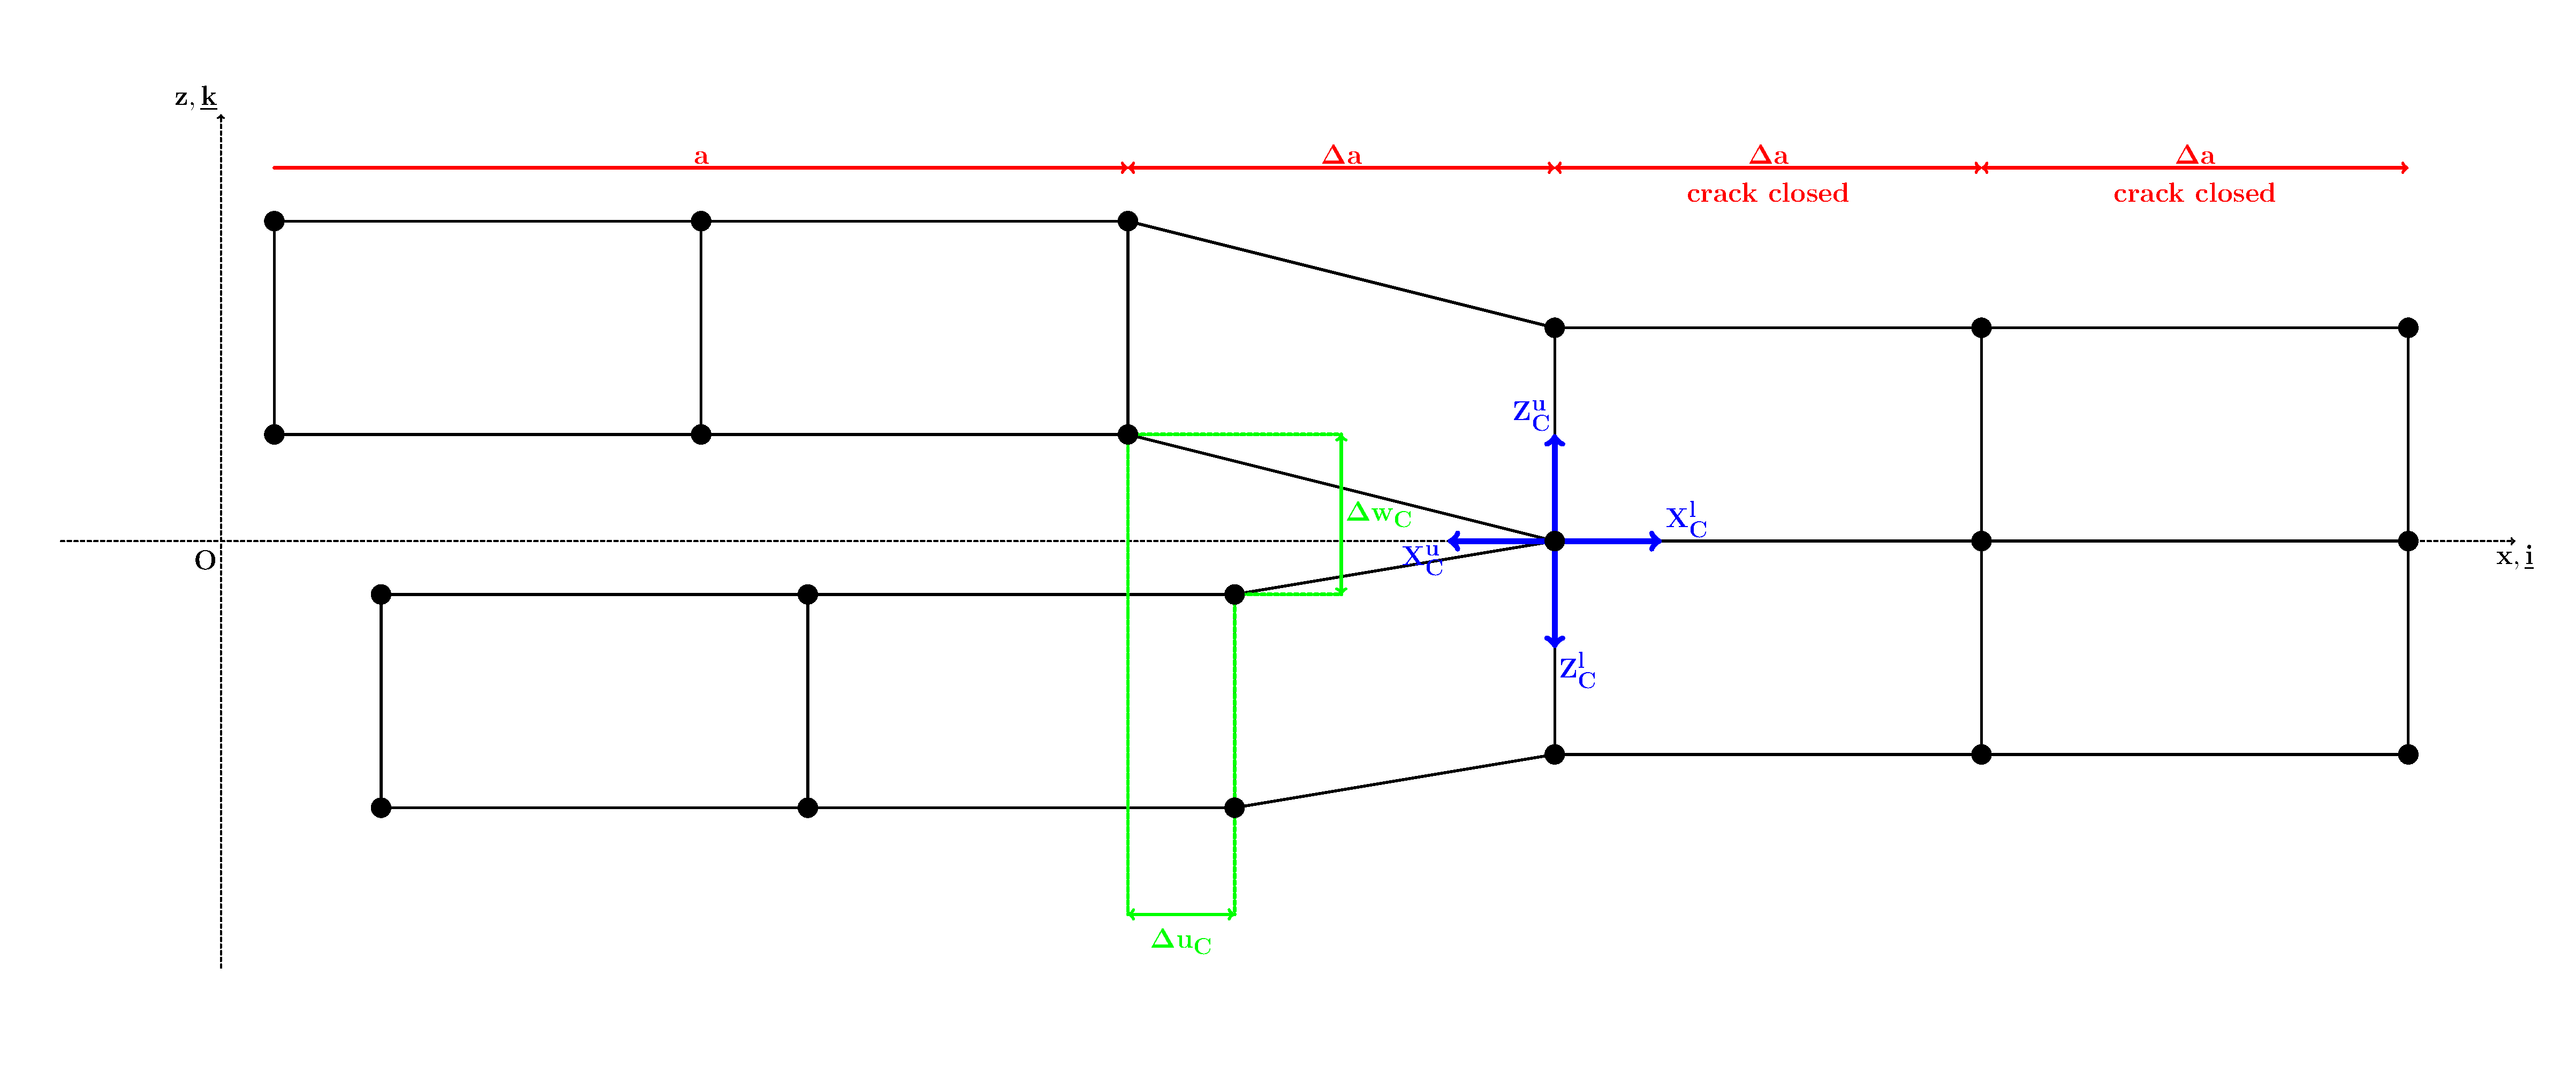
\includegraphics[width=\columnwidth]{VCCT.pdf}
 % \caption{VCCT}
  \label{fig:vcct}
\end{figure}

\begin{equation*}
G_{I}=\frac{Z_{C}\Delta w_{C}}{2B\Delta a}\quad G_{II}=\frac{X_{C}\Delta u_{C}}{2B\Delta a}
\end{equation*}

\end{itemize}
\end{column}
\begin{column}{0.5\textwidth}
\centering
\begin{itemize}[label=\ding{212}]
\item J-Integral

\begin{figure}
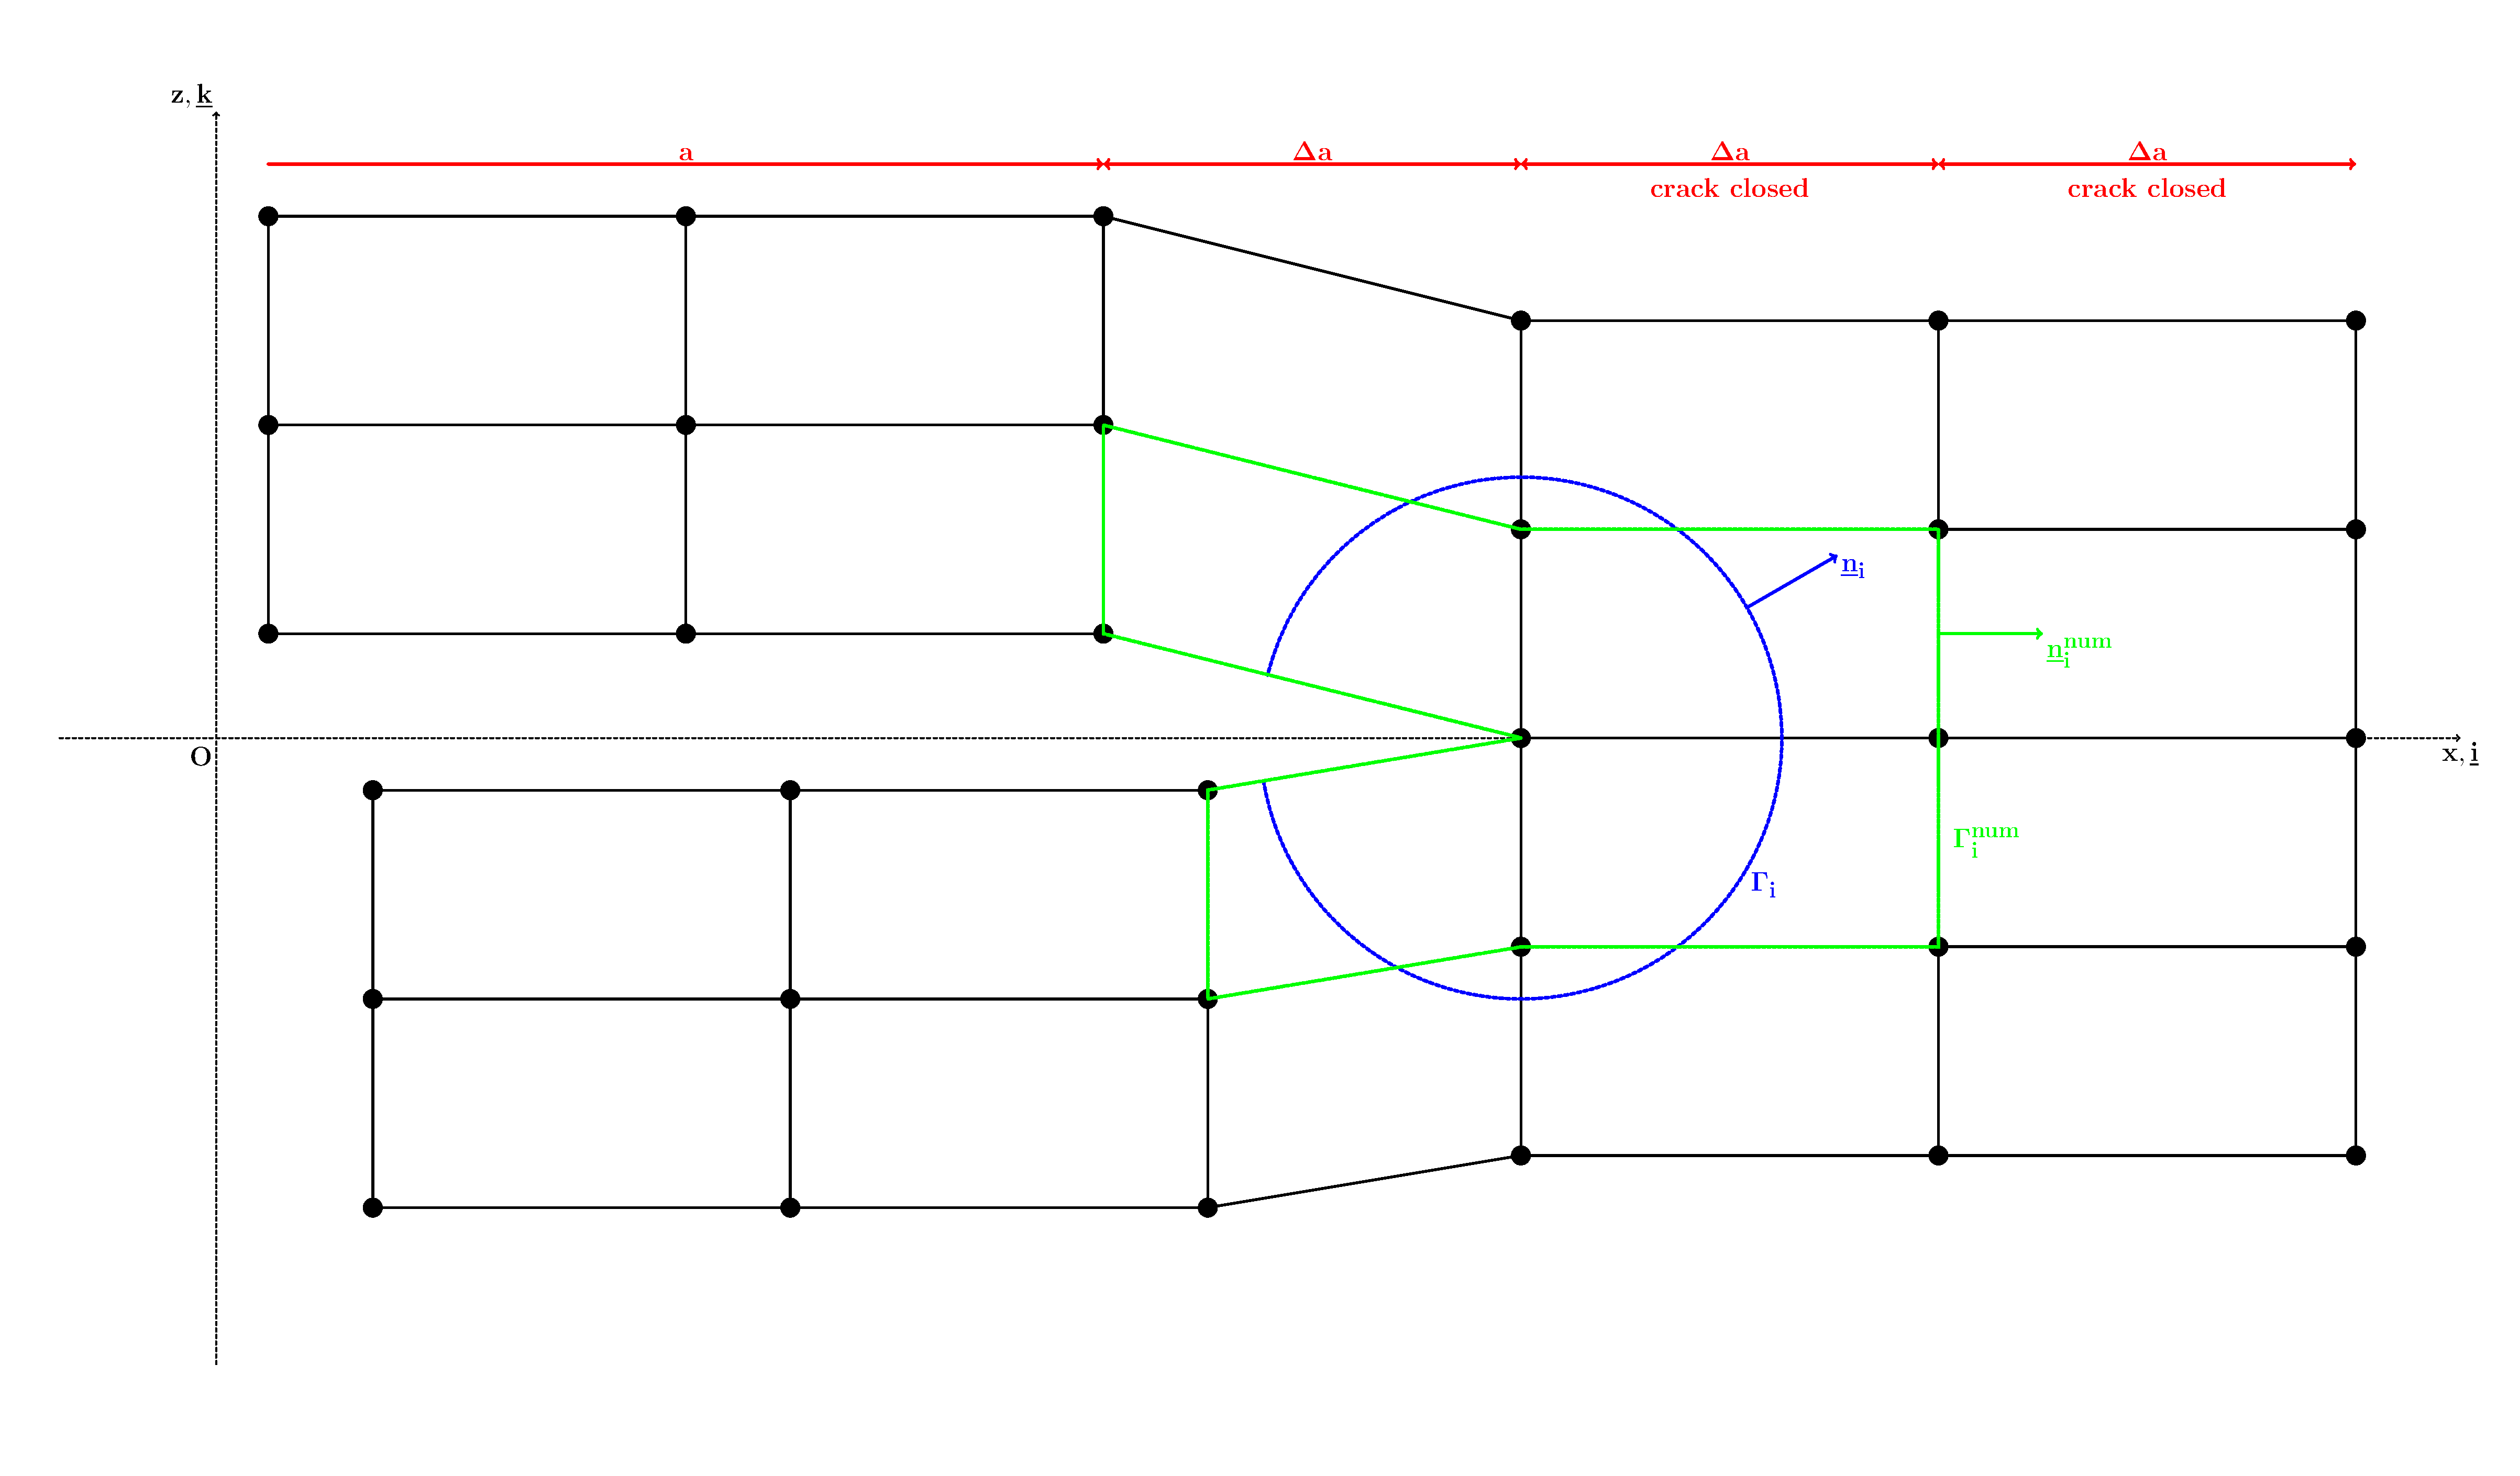
\includegraphics[width=\columnwidth]{J-integral.pdf}
 % \caption{Angular discretization at fiber/matrix interface.}
  \label{fig:jintegral}
\end{figure}

\begin{equation*}
J_{i}=\lim_{\varepsilon\to 0}\int_{\Gamma_{\varepsilon}}\left(W\left(\Gamma\right)n_{i}-n_{j}\sigma_{jk}\frac{\partial u_{k}\left(\Gamma,x_{i}\right)}{\partial x_{i}}\right)d\Gamma
\end{equation*}

\end{itemize}
\end{column}
\end{columns}
\end{frame}

\section[The Fiber-Matrix Interface Problem in FRPC]{The Fiber-Matrix Interface Problem in Fiber Reinforced Polymer Laminates}

\subsection{From macro to micro}

\begin{frame}
\frametitle{From macro to micro}
\vspace{-1cm}
\centering
\begin{figure}
\centering
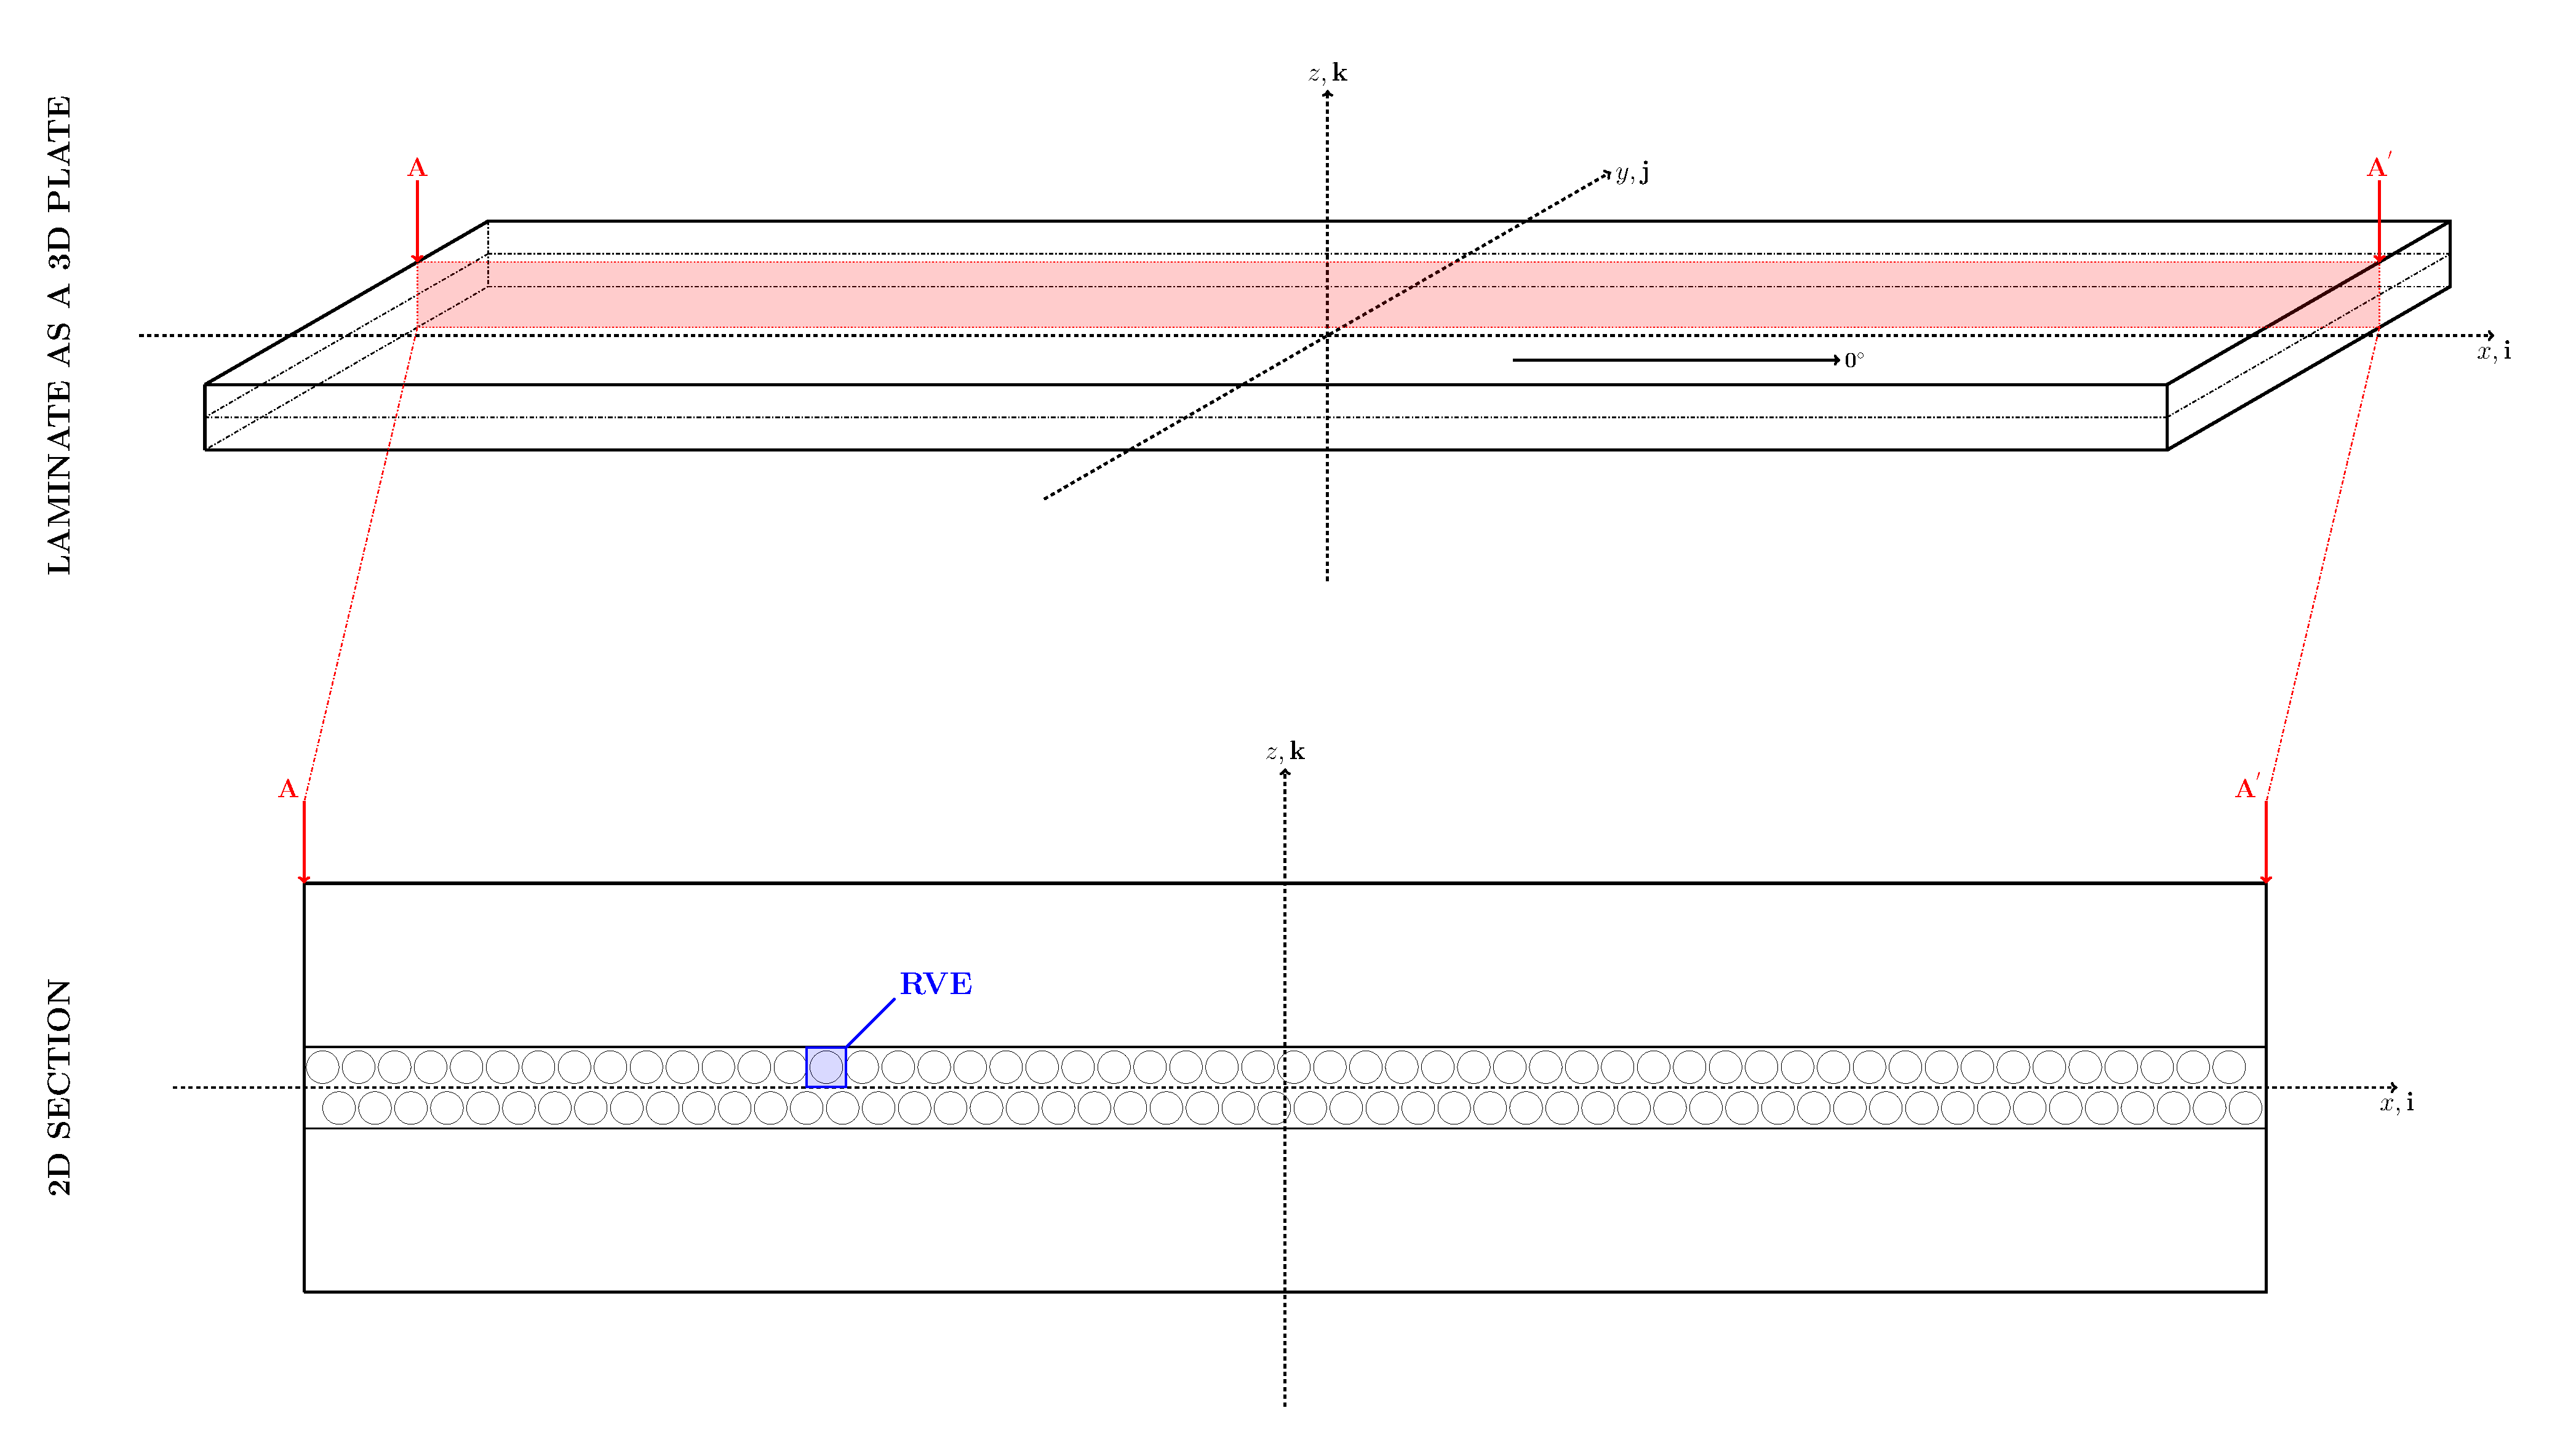
\includegraphics[height=0.8\textheight]{laminate-section.pdf}
%\caption{}
\label{fig:spread-tow-schematic}
\end{figure}
\end{frame}

\subsection{The Fiber-Matrix Interface Crack Problem}

\begin{frame}
\frametitle{\small The Fiber-Matrix Interface Crack Problem}
\vspace{-0.5cm}
\centering
\begin{columns}
\begin{column}{0.4\textwidth}
\begin{figure}
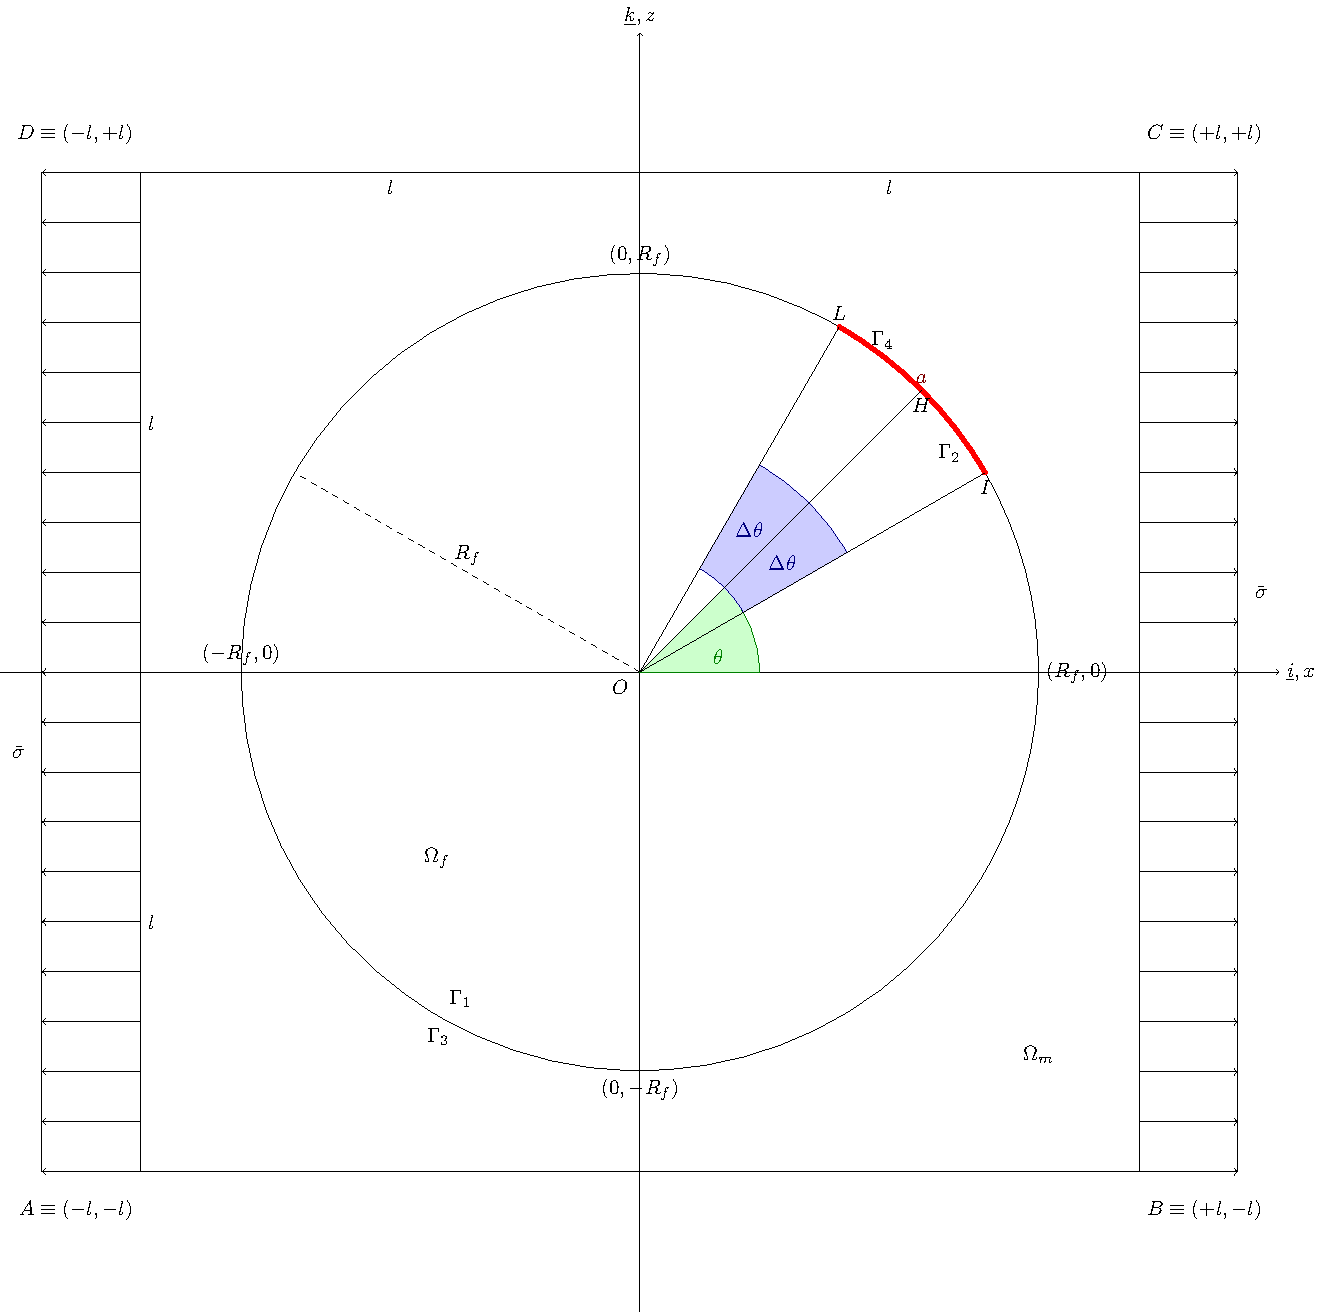
\includegraphics[width=\columnwidth]{fiberMatrixInterfaceProblem.pdf}
 % \caption{Angular discretization at fiber/matrix interface.}
  \label{fig:jintegral}
\end{figure}
\end{column}
\begin{column}{0.6\textwidth}
\footnotesize
\begin{table}
\begin{tabularx}{\columnwidth}{XXX}
&{\tiny \bf{Analytical}}&{\tiny \bf{Numerical}}\\
\midrule
{\tiny \textit{Method}}&{\tiny Analytical (complex) functions}&{\tiny FEM}\\
\midrule
{\tiny \textit{Domain Type}}&{\tiny Continuous}&{\tiny Discrete}\\
{\tiny \textit{Domain Size}}&{\tiny Infinite}&{\tiny Finite}\\
\midrule
{\tiny \textit{Natural variable}}&{\tiny Stress (stress function)}&{\tiny Displacement field}\\
{\tiny \textit{Conjugate variable}}&{\tiny Displacement}&{\tiny Stress}\\
\midrule
{\tiny \textit{Dirichlet BC}}&{\tiny Stress}&{\tiny Displacement}\\
{\tiny \textit{Loading process}}&{\tiny Force-controlled}&{\tiny Displacement-controlled}\\
\end{tabularx}
\end{table}
\end{column}
\end{columns}
\end{frame}

\subsection{FEM Model of the Fiber-Matrix Interface Crack}

\begin{frame}
\frametitle{\small FEM Model of the Fiber-Matrix Interface Crack}
\vspace{-0.5cm}
\centering
\begin{columns}
\begin{column}{0.7\textwidth}
\begin{figure}
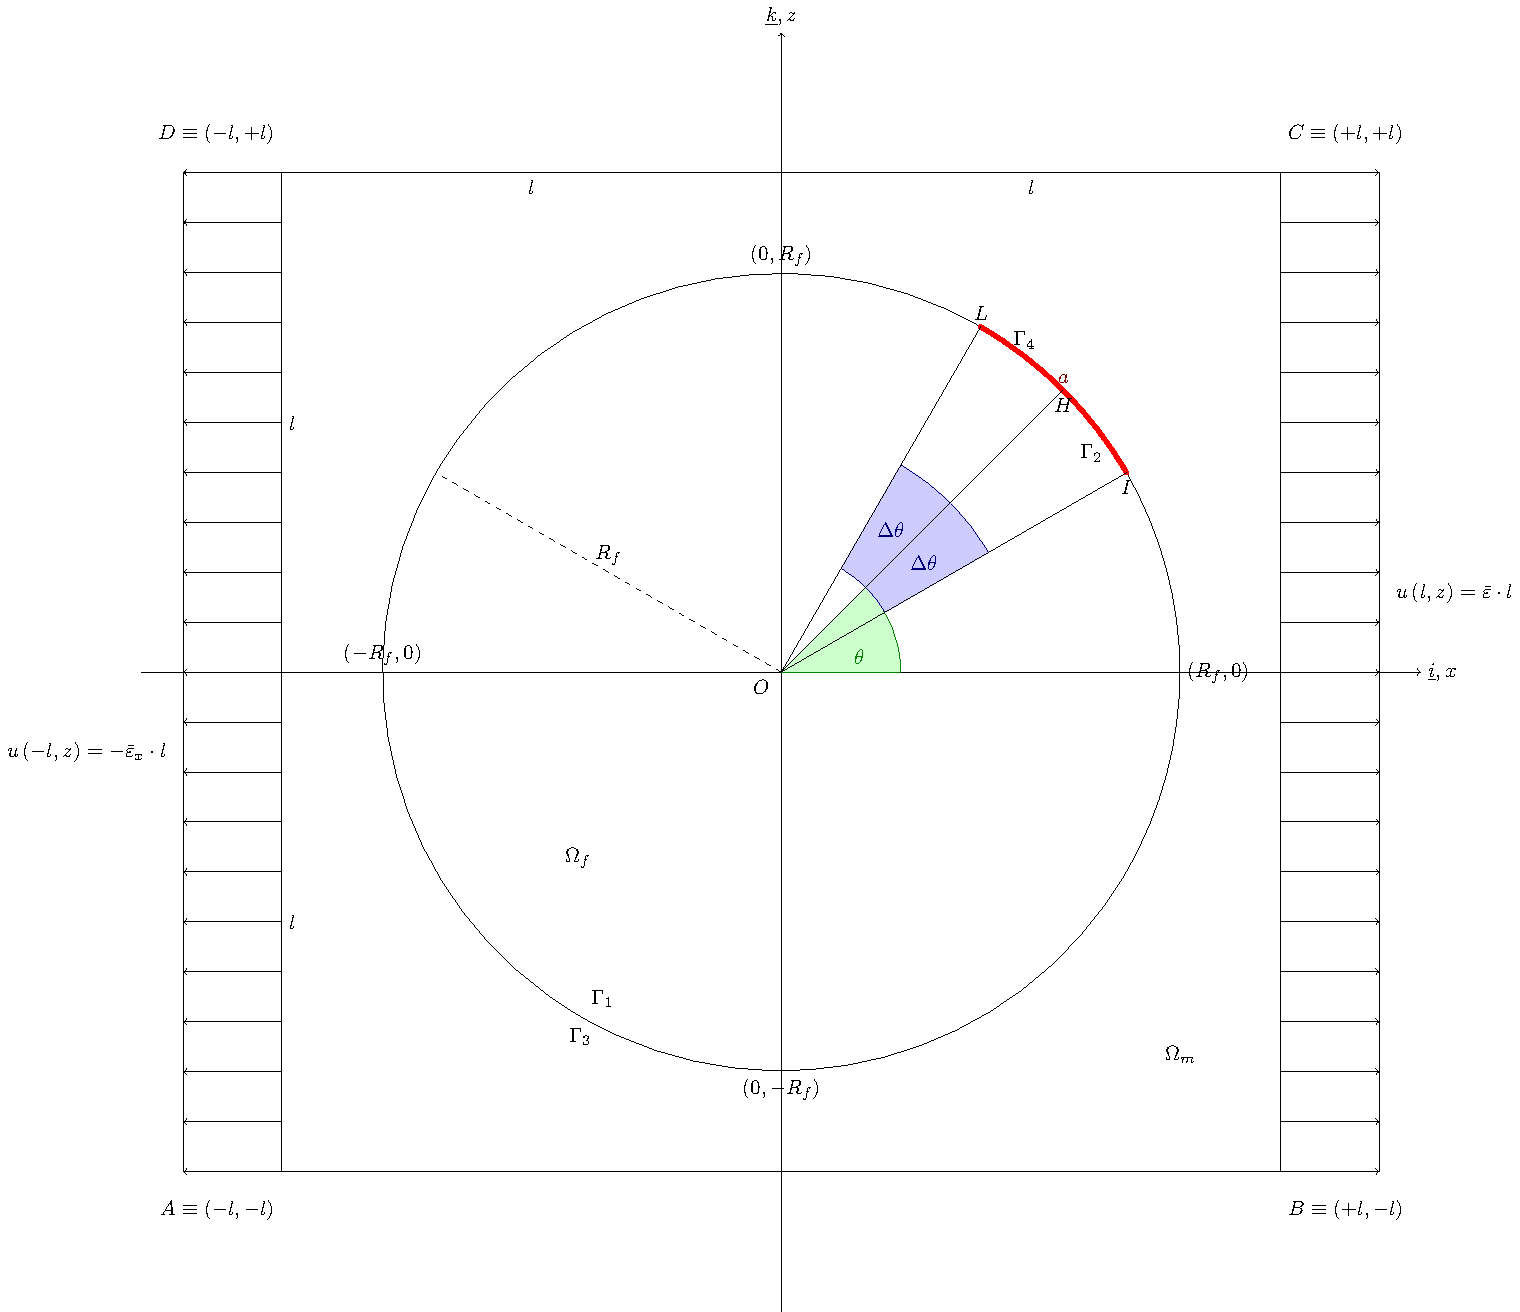
\includegraphics[width=\columnwidth]{FEMfiberMatrixInterfaceProblem.pdf}
 % \caption{Angular discretization at fiber/matrix interface.}
  \label{fig:jintegral}
\end{figure}
\end{column}
\begin{column}{0.3\textwidth}
\scriptsize
\begin{itemize}[label=\ding{212}]
\item 2D space
\item Linear elastic materials
\item Displacement-controlled
\item Dirichlet-type BC
\item LEFM
\item Contact interaction
\item Bi-linear quadrilateral elements
\end{itemize}
\end{column}
\end{columns}
\end{frame}

\section[Mesh \& Domain Size]{Effects of Mesh Refinement \& Domain Size}

\subsection{Domain size effect on $G_{0}$}

\begin{frame}
\frametitle{\small $G_{0}$ for $Vf_{f}=0.001$, $\frac{L}{R_{f}}\sim 28$, $\delta=0.4^{\circ}$}
\vspace{-0.5cm}
\begin{figure}
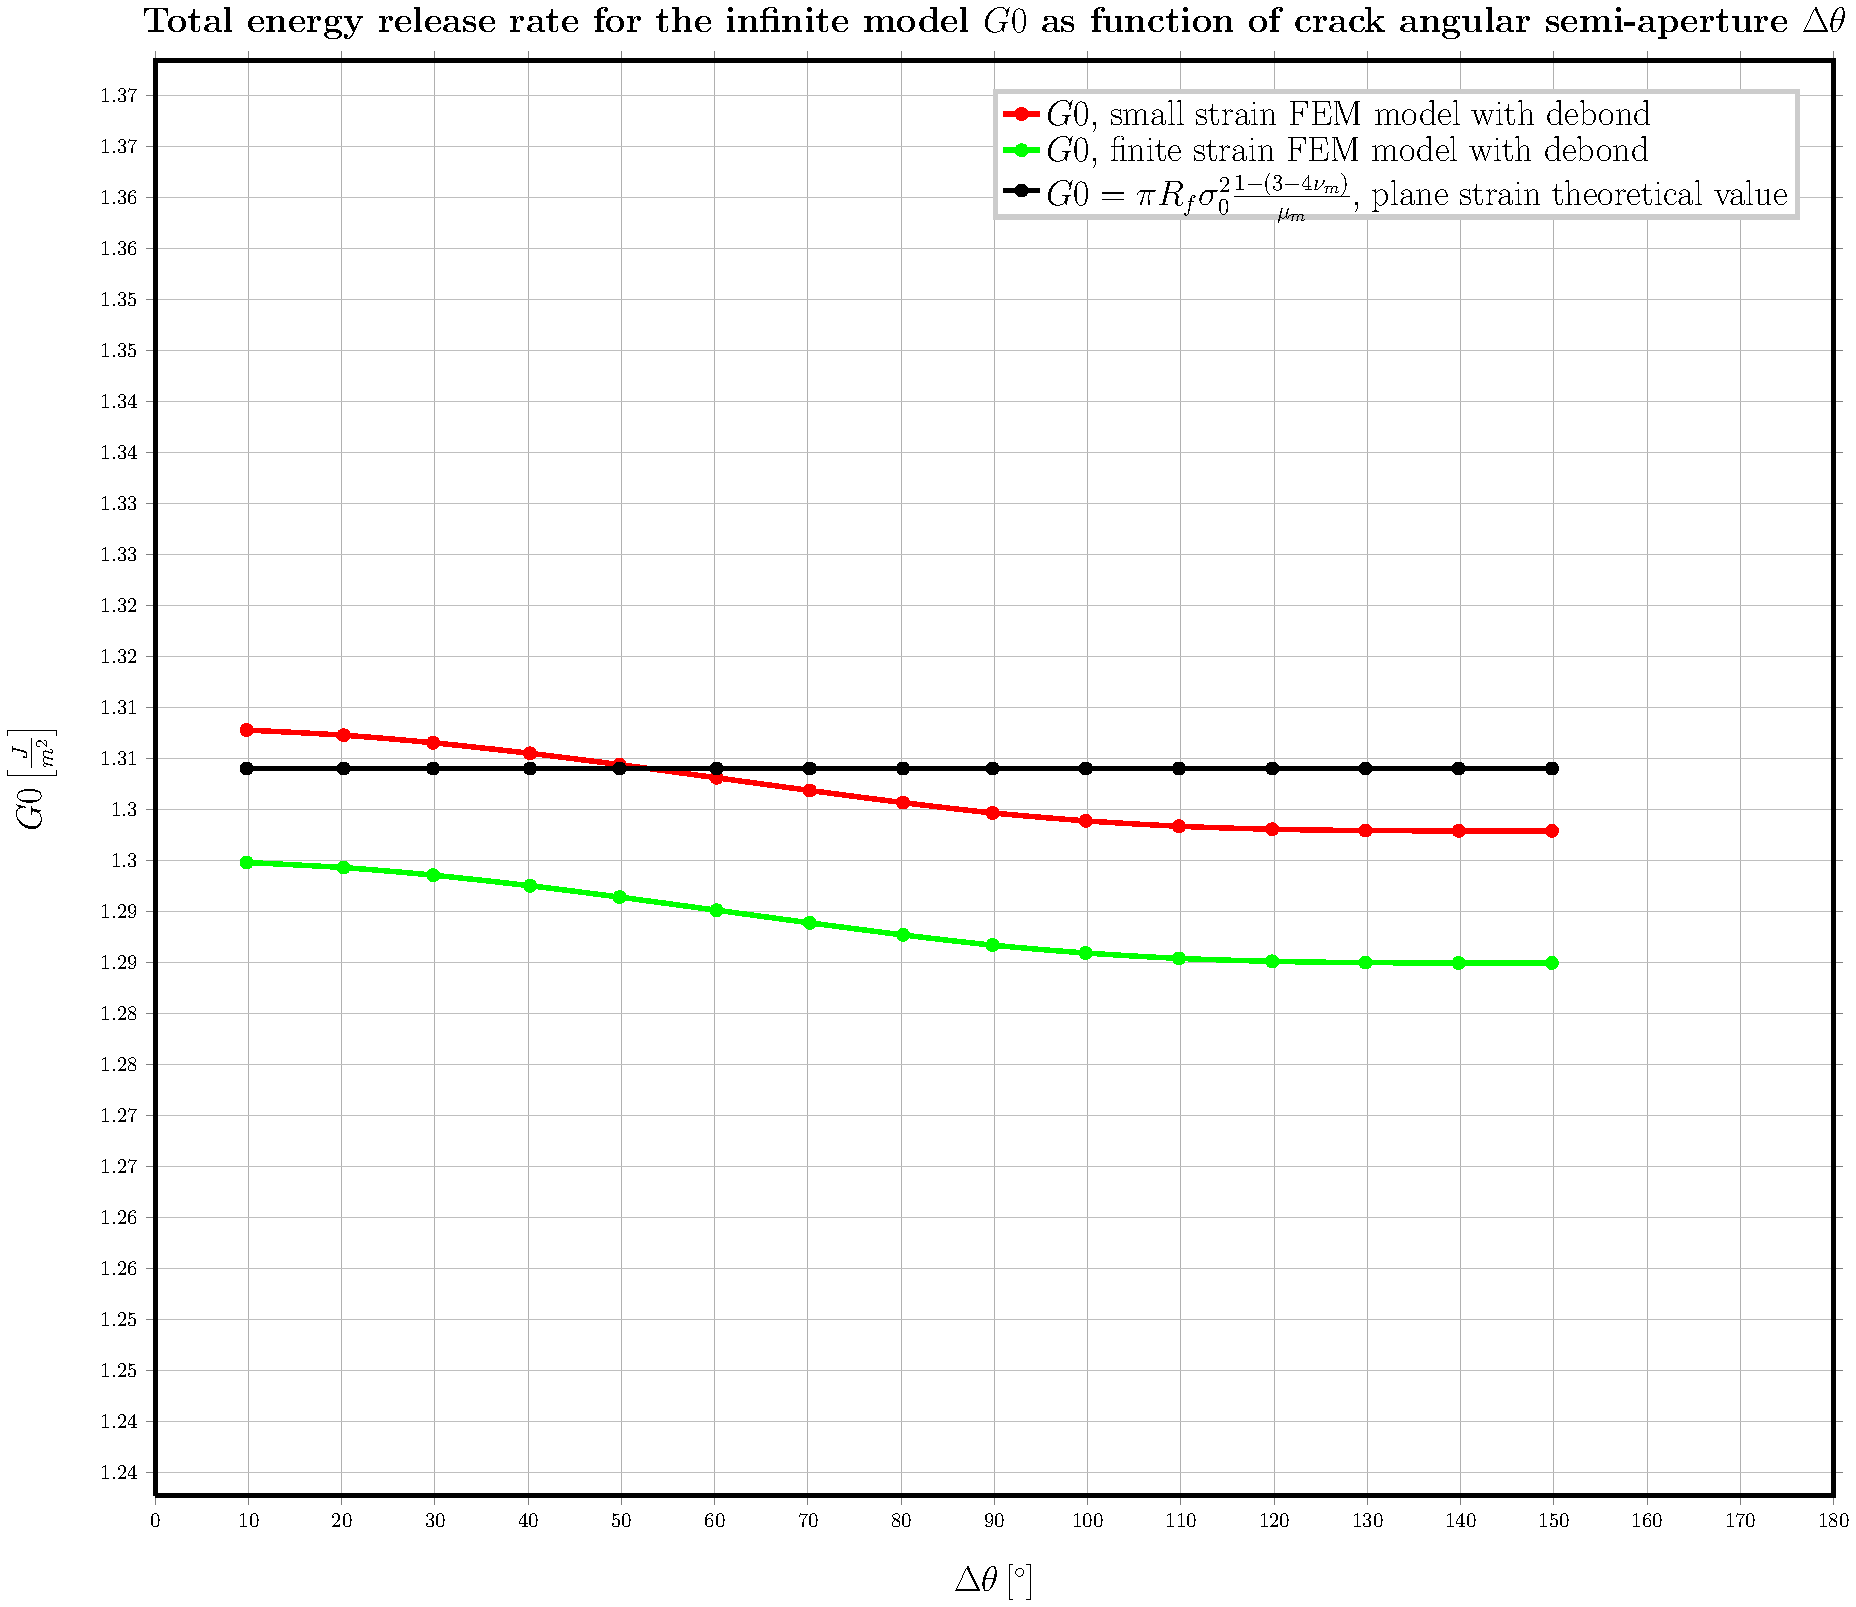
\includegraphics[height=0.7\textheight]{2017-06-23_AbqRunSummary_SingleFiberEqRfSmallFiniteStrain_G0_Summary.pdf}
 \caption{In red small strain FEM, in green finite strain FEM, in black $G_{0}$ calculated assuming $\sigma_{0}=\frac{E}{1-\nu^ 2}\varepsilon$.}
  \label{fig:jintegral}
\end{figure}
\end{frame}

\begin{frame}
\frametitle{\small $G_{0}$ for $Vf_{f}=0.000079$, $\frac{L}{R_{f}}\sim 100$, $\delta=0.4^{\circ}$}
\vspace{-0.5cm}
\begin{figure}
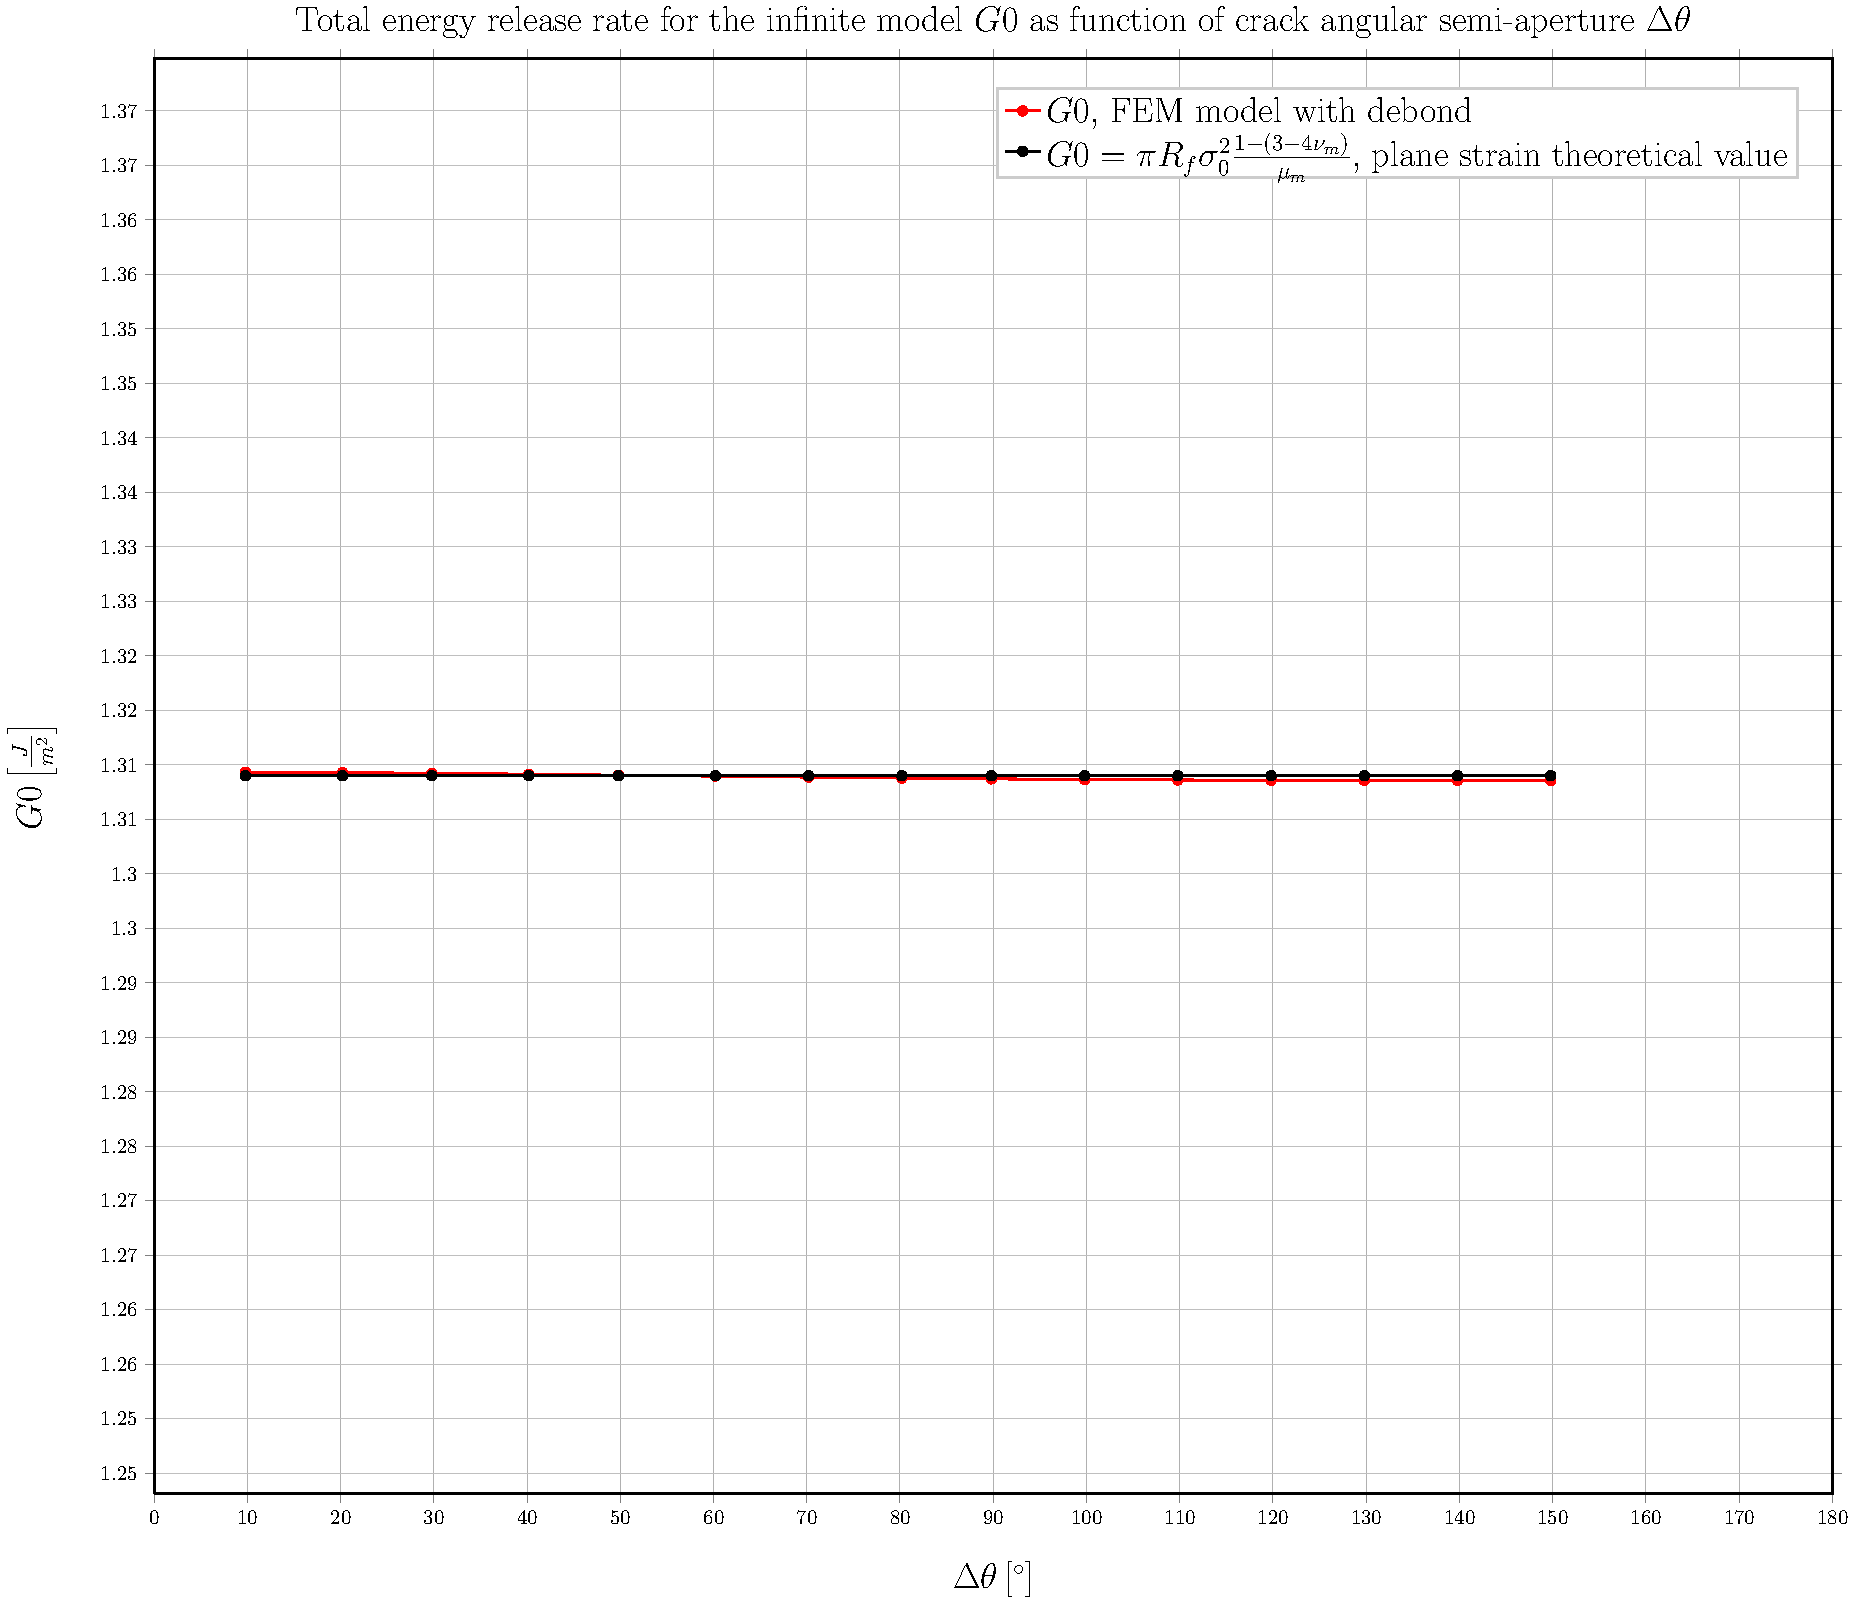
\includegraphics[height=0.7\textheight]{2017-06-16_AbqRunSummary_SingleFiberEqRfSmallStrain-D0-4_G0_Summary.pdf}
 \caption{In red small strain FEM, in green finite strain FEM, in black $G_{0}$ calculated assuming $\sigma_{0}=\frac{E}{1-\nu^ 2}\varepsilon$.}
  \label{fig:jintegral}
\end{figure}
\end{frame}

\subsection{Mesh refinement effect on mode ratio}

\begin{frame}
\frametitle{\small $G_{I}$, VCCT, $Vf_{f}=0.000079$, $\frac{L}{R_{f}}\sim 100$}
\vspace{-0.5cm}
\centering
\captionsetup[figure]{font=scriptsize,labelfont=scriptsize}
\begin{figure}[!h]
\centering
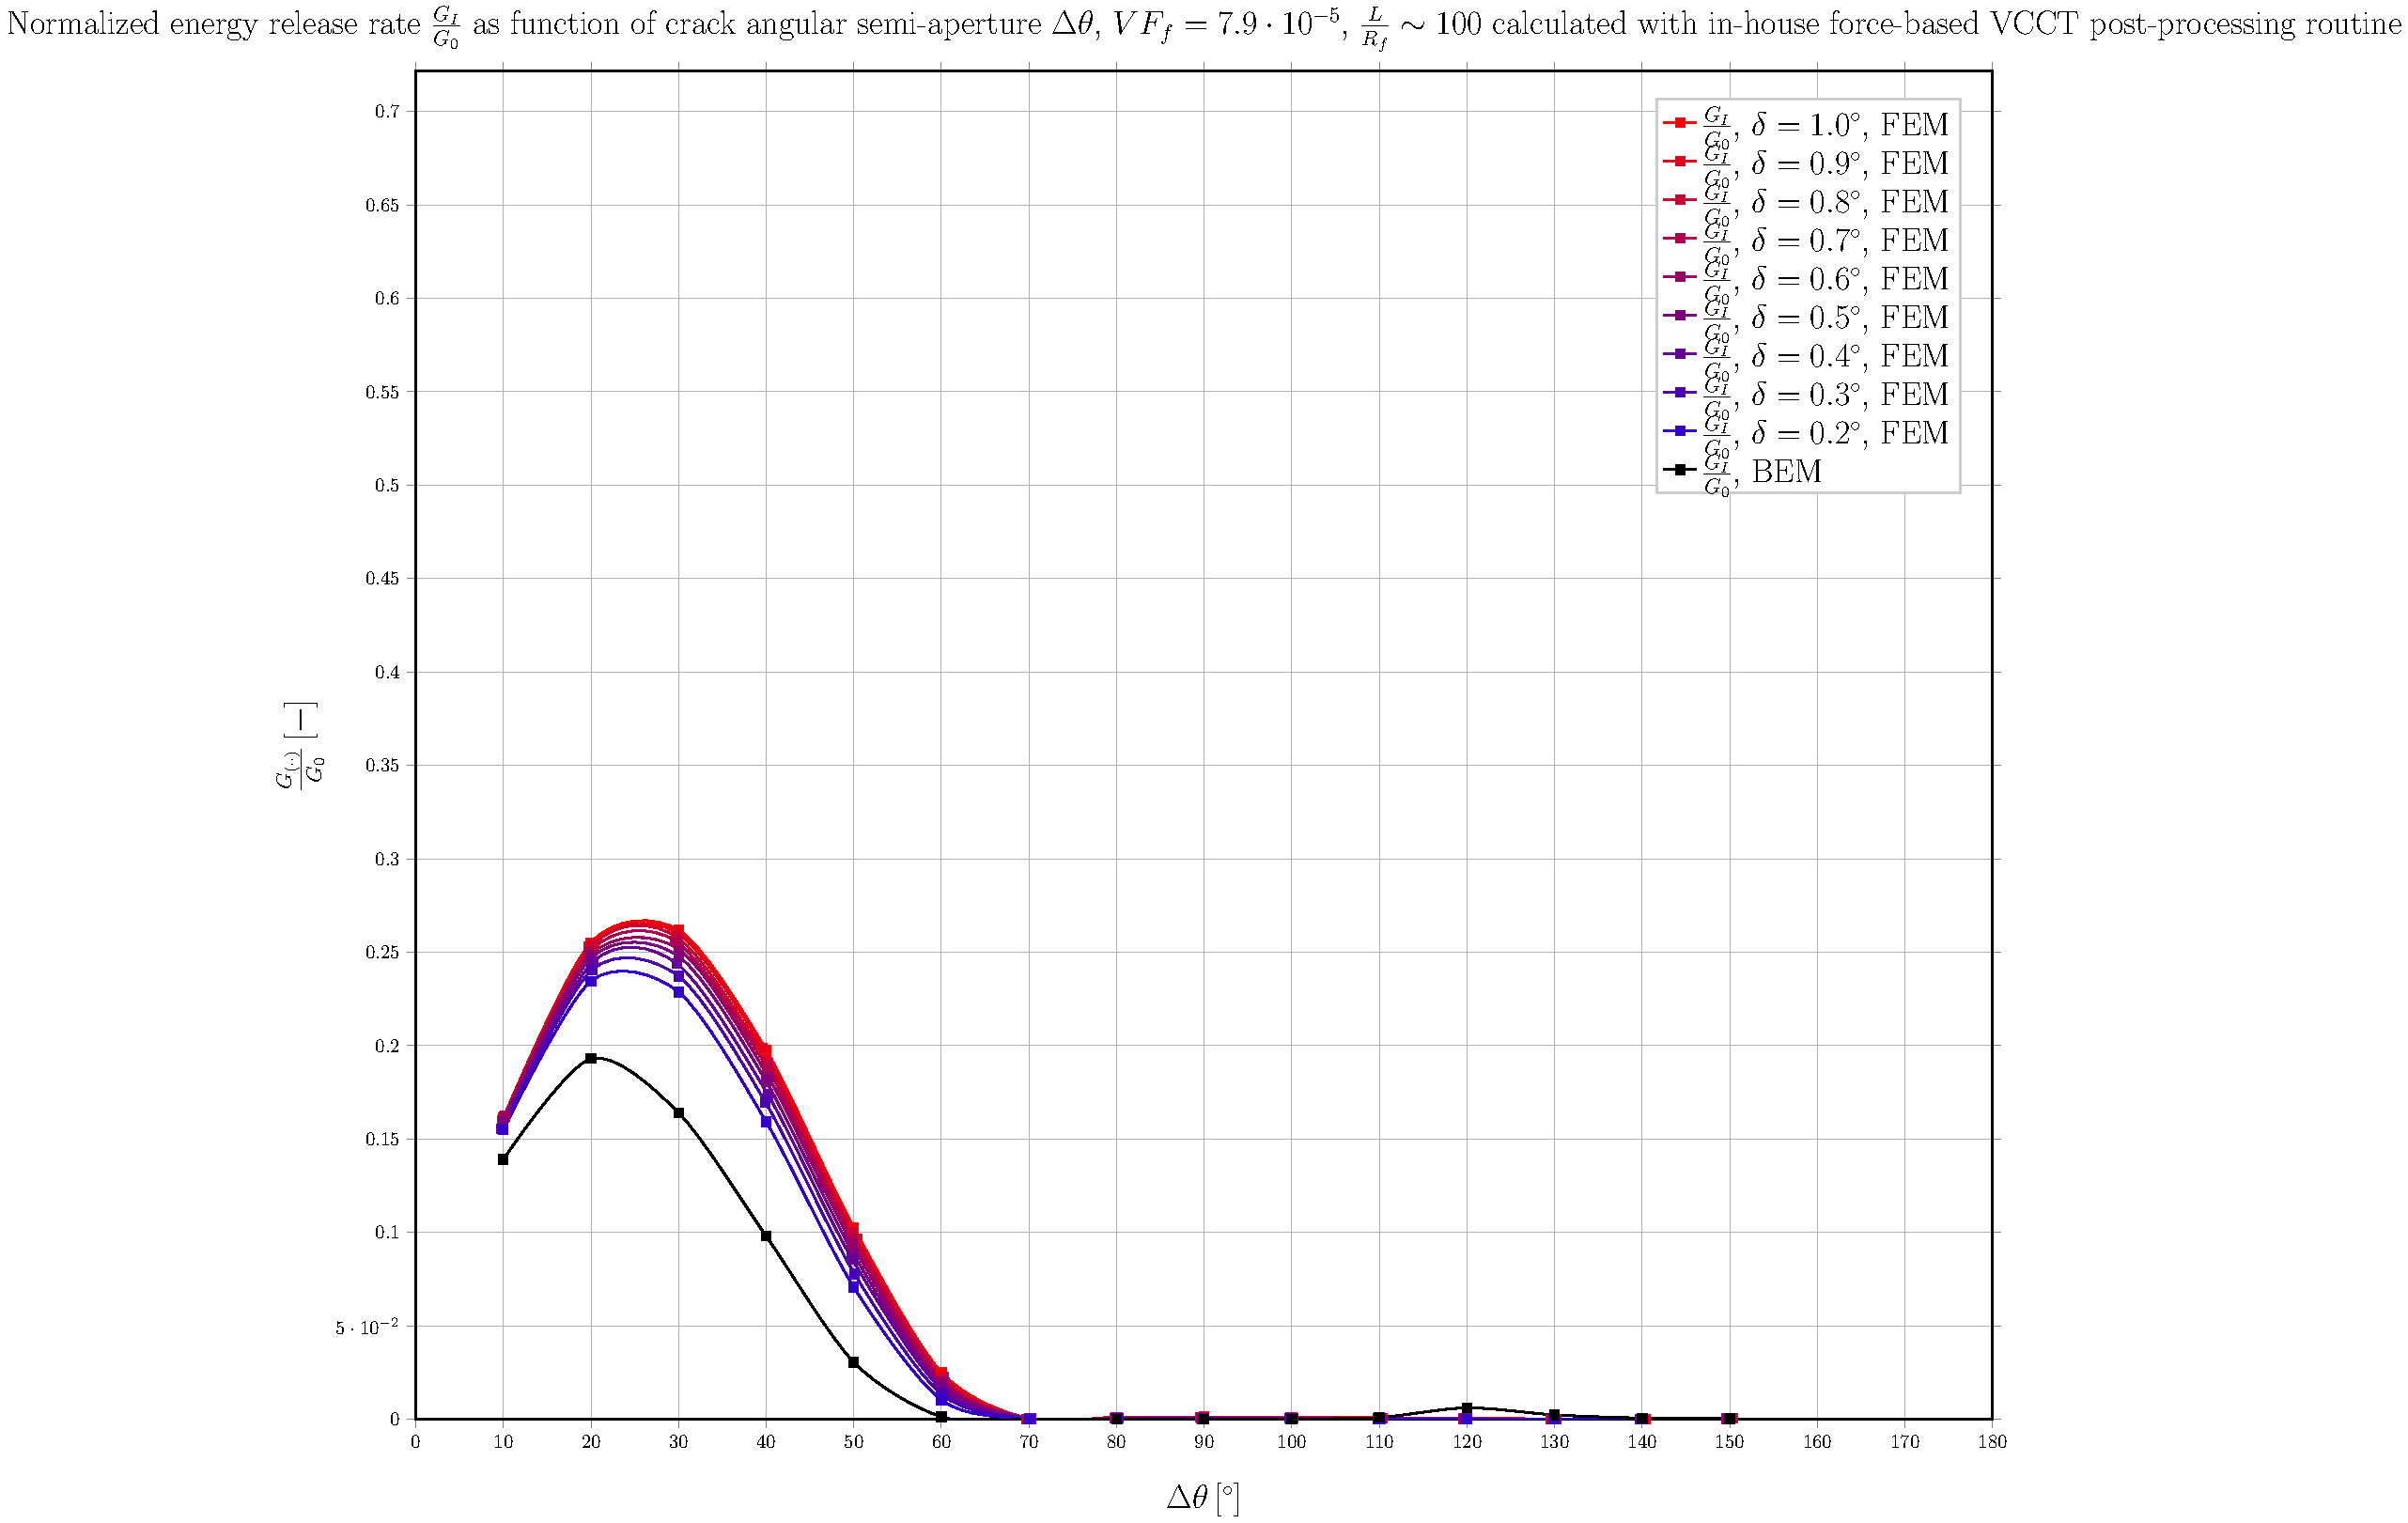
\includegraphics[height=0.7\textheight]{2017-07-10_AbqRunSummary_SmallStrain_M-F-VCCT_GI.pdf}
  \caption{\scriptsize Fading from red to blue for decreasing size of elements at the interface, VCCT from FEM results; in black BEM results.}
  \label{fig:res1}
\end{figure}
\end{frame}

\begin{frame}
\frametitle{\small $G_{II}$, VCCT, $Vf_{f}=0.000079$, $\frac{L}{R_{f}}\sim 100$}
\vspace{-0.5cm}
\centering
\captionsetup[figure]{font=scriptsize,labelfont=scriptsize}
\begin{figure}[!h]
\centering
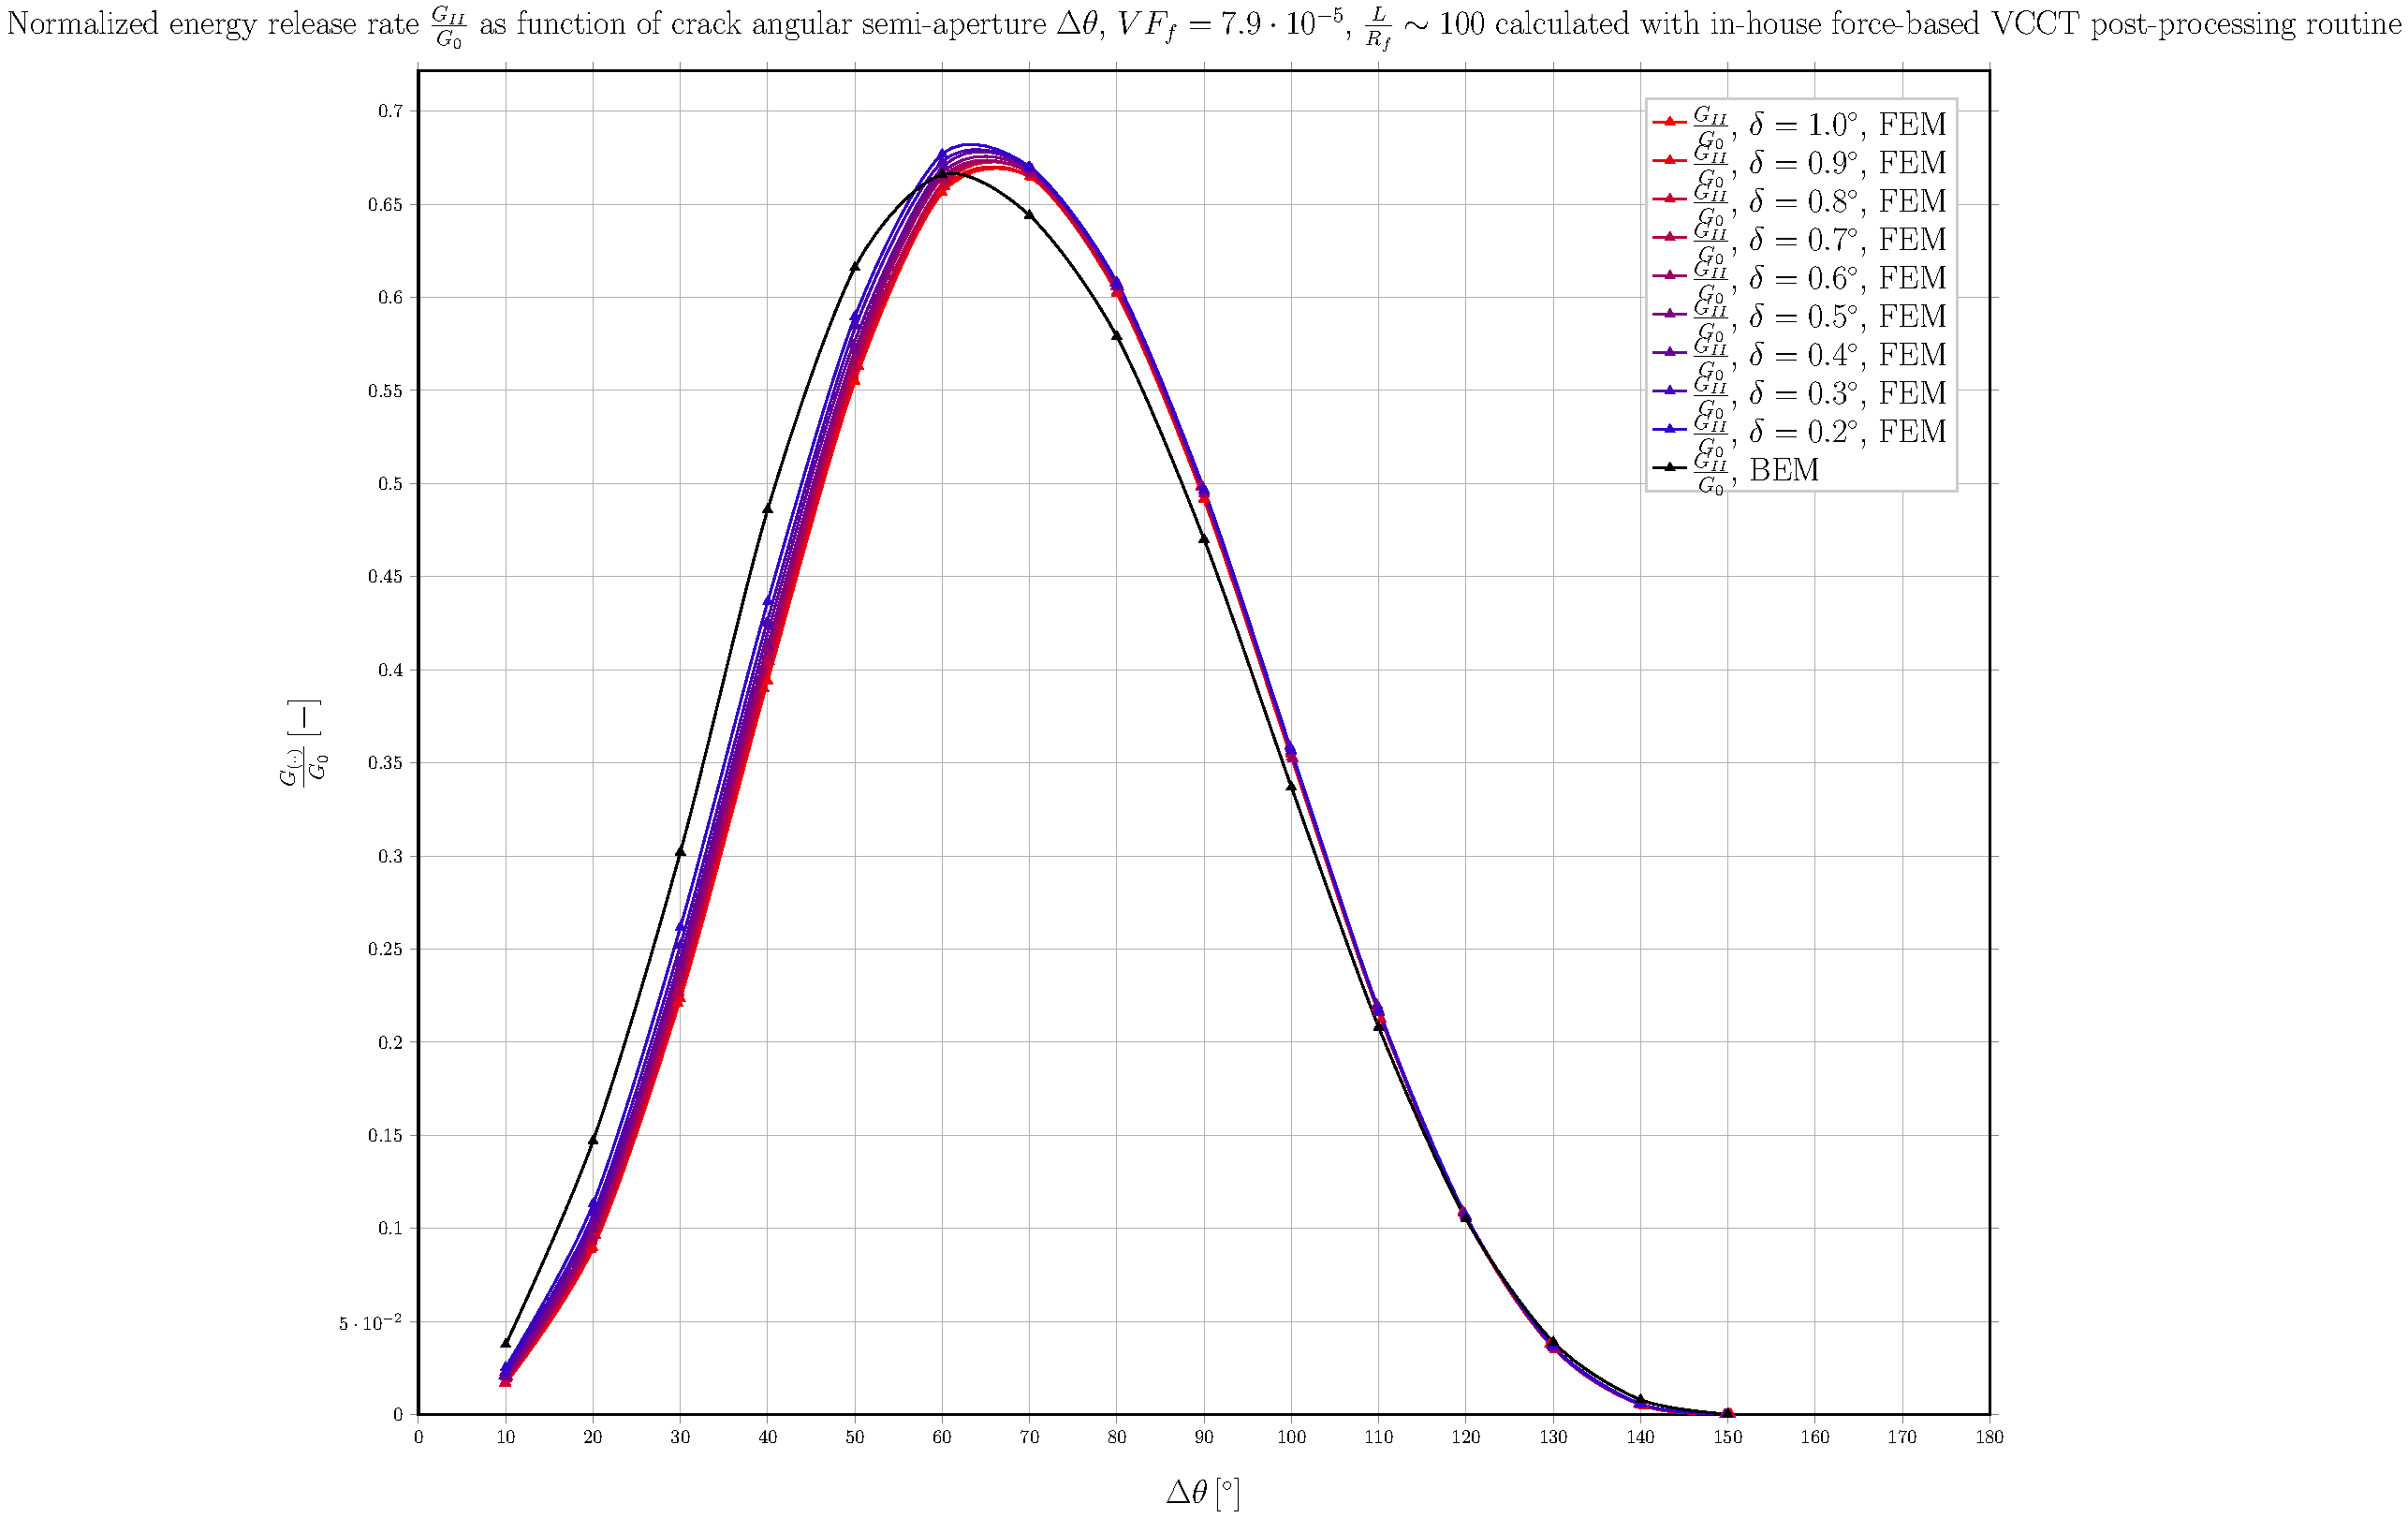
\includegraphics[height=0.7\textheight]{2017-07-10_AbqRunSummary_SmallStrain_M-F-VCCT_GII.pdf}
  \caption{\scriptsize Fading from red to blue for decreasing size of elements at the interface, VCCT from FEM results; in black BEM results.}
  \label{fig:res1}
\end{figure}
\end{frame}

\begin{frame}
\frametitle{\small $G_{TOT}$, VCCT, $Vf_{f}=0.000079$, $\frac{L}{R_{f}}\sim 100$}
\vspace{-0.5cm}
\centering
\captionsetup[figure]{font=scriptsize,labelfont=scriptsize}
\begin{figure}[!h]
\centering
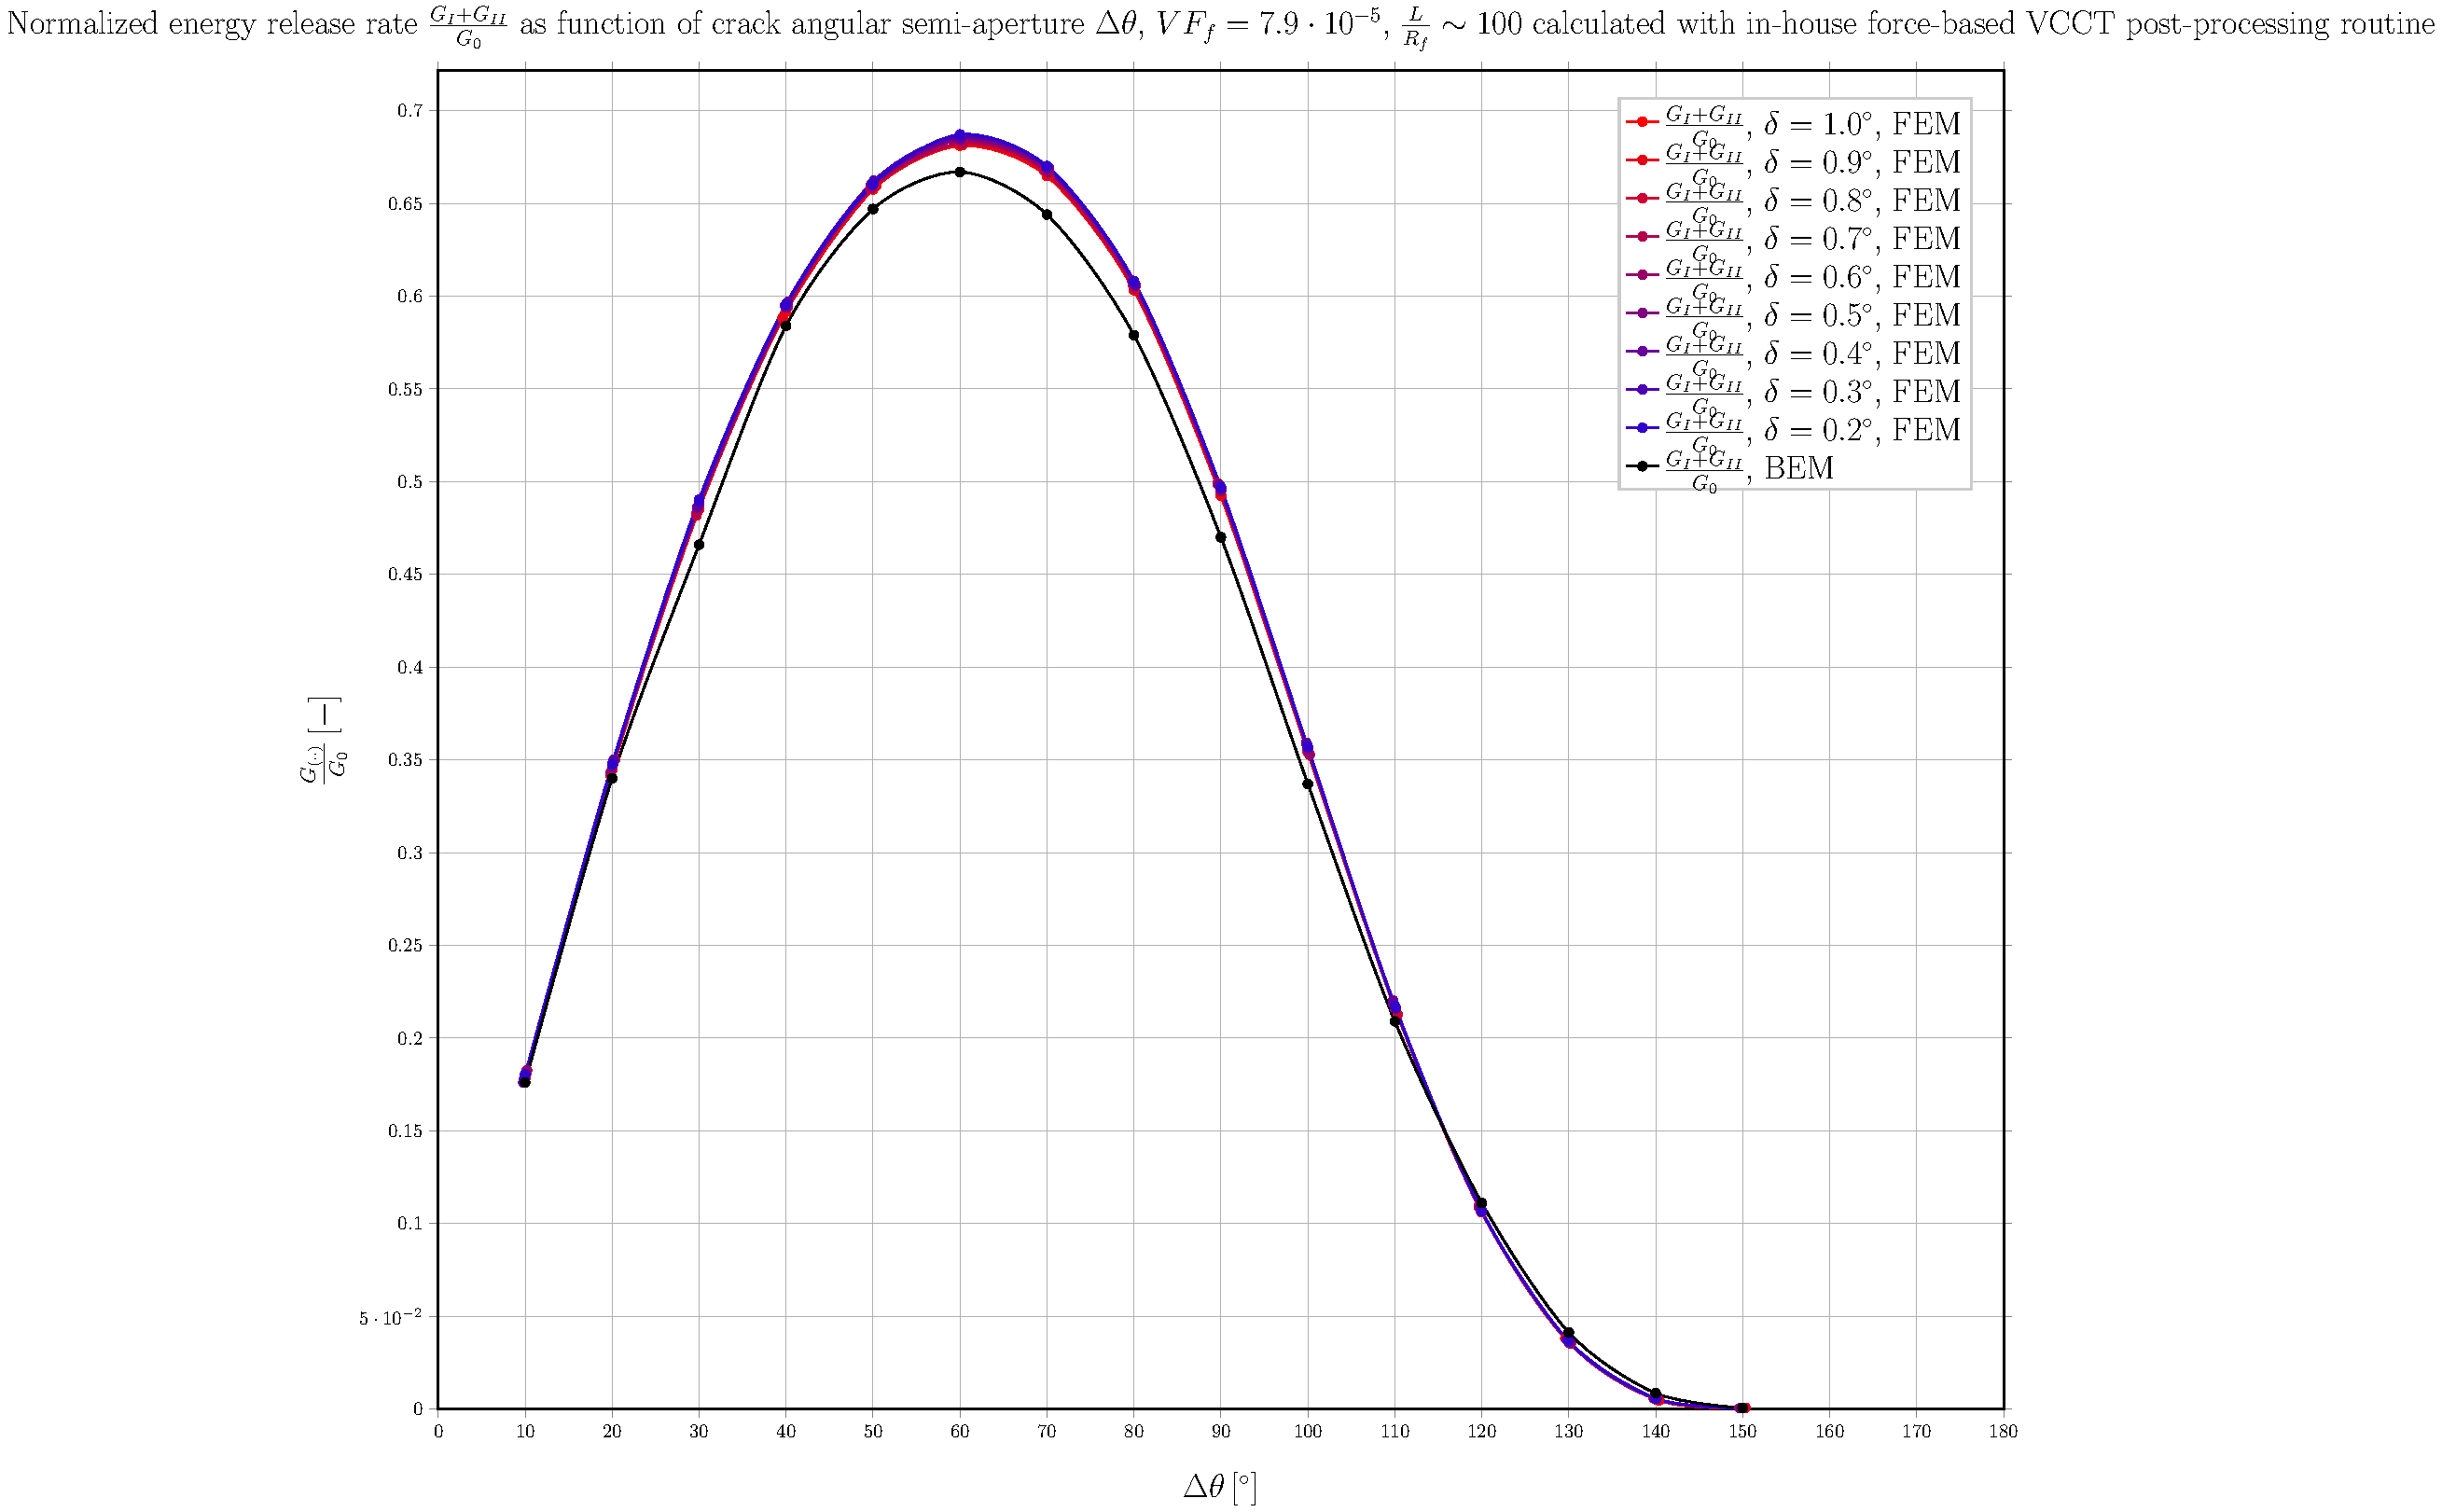
\includegraphics[height=0.7\textheight]{2017-07-10_AbqRunSummary_SmallStrain_M-F-VCCT_GTOT.pdf}
  \caption{\scriptsize Fading from red to blue for decreasing size of elements at the interface, VCCT from FEM results; in black BEM results.}
  \label{fig:res1}
\end{figure}
\end{frame}

\section[Conclusions]{Conclusions \& Outlook}

\begin{frame}
\frametitle{\vspace*{0.5cm} Conclusions \& Outlook}
\vspace{-0.75cm}
\centering
\scriptsize
\begin{alertblock}{\footnotesize \bf{Conclusions}}
\begin{itemize}[label=\ding{212}]
  \item Domain size is a fundamental parameter in determining the RVE behaviour between finite and efffectively infinite size
	\item Mesh refinement affects directly mode ratio, increasing mode I with respect to mode II
\end{itemize}
\end{alertblock}
\begin{alertblock}{\footnotesize \bf{Outlook}}
\begin{itemize}[label=\ding{212}]
	\item Analyze the dependence on $\delta$ for $\frac{L}{R_{f}}=200,300,\dots$\\[9pt]
	\item Analyze the dependence on $\frac{L}{R_{f}}$ for constant $\delta$\\[9pt]
	\item Study finite size effects
\end{itemize}
\end{alertblock}
\end{frame}

%\section{Appendices \& References}

%\subsection{Appendices}

%\begin{frame}[label=]
%\frametitle{}
%\end{frame}



%\begin{frame}
%\frametitle{\small Evaluation of $G_{0}$}
%\vspace{-0.7cm}
%\footnotesize
%\centering
%\captionsetup[figure]{font=scriptsize,labelfont=scriptsize}
%\begin{equation}
%G_{0}=\pi R_{f}\sigma^{2}_{0}\frac{1+k_{m}}{8G_{m}}
%\end{equation}
%\begin{equation}
%k_{m}=3-4\nu_{m}
%\end{equation}
%\begin{equation}
%\sigma_{0}^{undamaged}=\frac{E_{m}}{1-\nu^{2}_{m}}\varepsilon_{xx}
%\end{equation}%
%\end{frame}


%\section{References}

%\begin{frame}[t,label=references,allowframebreaks]
%       \frametitle{References}
%	\begin{itemize}
%%	\item Loading rate effects on delamination:\\[10pt] \textit{Loading\_rate\_effects\_on\_CFRP.bib}\\[30pt]
%	\item Body-fitted grids for FSI modeling with LBM:\\[10pt] %\textit{Fluid\_structure\_interaction\_on\_deformable\_surfaces.bib}
%	\end{itemize}
%        \bibliographystyle{amsalpha}
%        {\footnotesize
%          \bibliography{PSI_talk.bib}
%        }
        %\bibliography{/auto.mounter/home/lucadistasio/Documents/ETH/Research_material/References/fsi_references_kbib.bib}
%\end{frame}

%\subsection{References}

%\begin{frame}[allowframebreaks]
%  \frametitle{References}

%  \begin{thebibliography}{10}

%  \beamertemplatebookbibitems
%  % Start with overview books.
%
%  \bibitem{Author1990}
%    A.~Author.
%    \newblock {\em Handbook of Everything}.
%    \newblock Some Press, 1990.


%  \beamertemplatearticlebibitems
  % Followed by interesting articles. Keep the list short.


%  \end{thebibliography}
%\end{frame}

\begin{frame}[plain]
\frametitle{}
\end{frame}

\end{document}
